%% LyX 2.0.3 created this file.  For more info, see http://www.lyx.org/.
%% Do not edit unless you really know what you are doing.
\documentclass[twoside,english]{paper}
\usepackage{lmodern}
\renewcommand{\ttdefault}{lmodern}
\usepackage[T1]{fontenc}
\usepackage[latin9]{inputenc}
\usepackage[a4paper]{geometry}
\geometry{verbose,tmargin=3cm,bmargin=2.5cm,lmargin=2cm,rmargin=2cm}
\usepackage{color}
\usepackage{babel}
\usepackage{float}
\usepackage{bm}
\usepackage{amsthm}
\usepackage{amsmath}
\usepackage{amssymb}
\usepackage{graphicx}
\usepackage{esint}
\usepackage[unicode=true,pdfusetitle,
 bookmarks=true,bookmarksnumbered=false,bookmarksopen=false,
 breaklinks=false,pdfborder={0 0 0},backref=false,colorlinks=false]
 {hyperref}
\usepackage{breakurl}
\usepackage{makeidx}

\makeatletter

%%%%%%%%%%%%%%%%%%%%%%%%%%%%%% LyX specific LaTeX commands.
%% Because html converters don't know tabularnewline
\providecommand{\tabularnewline}{\\}

%%%%%%%%%%%%%%%%%%%%%%%%%%%%%% Textclass specific LaTeX commands.
\numberwithin{equation}{section}
\numberwithin{figure}{section}

%%%%%%%%%%%%%%%%%%%%%%%%%%%%%% User specified LaTeX commands.
\usepackage{babel}

\@ifundefined{showcaptionsetup}{}{%
 \PassOptionsToPackage{caption=false}{subfig}}
\usepackage{subfig}
\makeatother

\usepackage{listings}


\begin{document}

\title{Generalised parton distributions}

\author{Valerio Bertone}

\tableofcontents{}

\section{Introduction}

In this set of notes I collect the technical aspects concerning
generalised parton distributions (GPDs). Since the computation GPDs
introduces new kinds of convolution integrals, a strategy aimed at
optimising the numerics needs to be devised.

\section{Evolution equation}

The evolution equation for GPDs reads:\footnote{It should be noticed
  that the integration bounds of the integration in
  Eq.~(\ref{eq:eveq}) are dictated by the operator defintion of the
  distribution $f$ on the light cone and not by the kernel
  $\mathbb{V}$.}
\begin{equation}
\mu^2\frac{d}{d\mu^2}f(x,\xi) =
\int_{-1}^{1}\frac{dx'}{\left|2\xi\right|}\mathbb{V}\left(\frac{x}{\xi},\frac{x'}{\xi}\right)f(x',\xi)\,.
\label{eq:eveq}
\end{equation}
In general, the GPD $f$ and the evolution kernel $\mathbb{V}$ should
be respectively interpreted as a vector and a matrix in flavour
space. However, for now, we will just be concerned with the integral
in the r.h.s. of Eq.~(\ref{eq:eveq}) regardless of the flavour
structure.

The support of the evolution kernel
$\mathbb{V}\left(\frac{x}{\xi},\frac{x'}{\xi}\right)$ is shown in
Fig.~\ref{fig:GPDIntDomain}.
\begin{figure}[h]
  \begin{centering}
    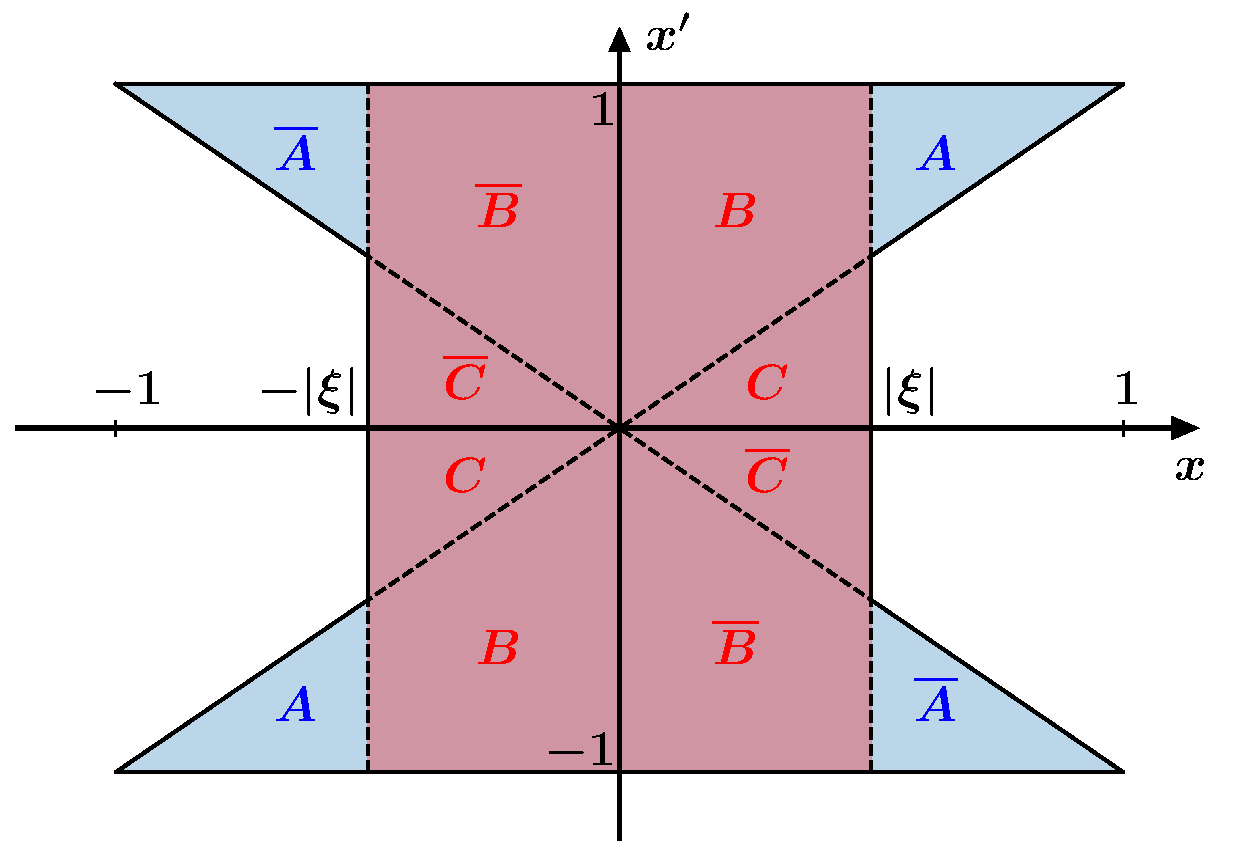
\includegraphics[width=0.7\textwidth]{plots/GPDIntDomain.pdf}
    \caption{Support domain of the evolution kernel.\label{fig:GPDIntDomain}}
  \end{centering}
\end{figure}
The knowledge of the support region of the evolution kernel allows us
to rearrange Eq.~(\ref{eq:eveq}) as follows:
\begin{equation}
\displaystyle\mu^2\frac{d}{d\mu^2}f(\pm x,\xi) =\int_{b(x)}^{1}\frac{dx'}{x'}\left[\frac{x'}{\left|2\xi\right|}\mathbb{V}\left(\pm \frac{x}{\xi},\frac{x'}{\xi}\right)f(x',\xi)+\frac{x'}{\left|2\xi\right|}\mathbb{V}\left(\mp \frac{x}{\xi},\frac{x'}{\xi}\right)f(-x',\xi)\right]\,,
\end{equation}
with:
\begin{equation}
b(x) = |x|\theta\left(\left|\frac{x}{\xi}\right|-1\right)\,,
\label{eq:lowintb}
\end{equation}
and where we have used the symmetry property of the evolution kernels:
$\mathbb{V}(y,y')=\mathbb{V}(-y,-y')$. In the unpolarised case, it is
useful to define:\footnote{Notice the seemingly unusual fact that
  $f^{+}$ is defined as difference and $f^{-}$ as sum of GPDs computed
  at opposite values of $x$. This can be understood from the fact
  that, in the forward limit, $f(-x)= -\overline{f}(x)$, \textit{i.e.}
  the PDF of a quark computed at $-x$ equals the PDF of the
  corresponding antiquark computed at $x$ with opposite sign. The
  opposite sign is absent in the longitudinally polarised case.}
\begin{equation}
\begin{array}{rcl}
\displaystyle f^{\pm}(x,\xi) &=&\displaystyle  f(x,\xi) \mp
                       f(-x,\xi)\,,\\
\\
\displaystyle \mathbb{V}^{\pm}(y,y') &=&\displaystyle  \mathbb{V}(y,y') \mp \mathbb{V}(-y,y')\,,
\end{array}
\label{eq:pmdef}
\end{equation}
so that the evolution equation for $f^{\pm}$ reads:
\begin{equation}
\displaystyle\mu^2\frac{d}{d\mu^2}f^{\pm}(x,\xi) = \int_{b(x)}^{1}\frac{dx'}{x'}\frac{x'}{\left|2\xi\right|}
                                                         \mathbb{V}^{\pm}\left(\frac{x}{\xi},\frac{x'}{\xi}\right)f^{\pm}(x',\xi)\,.
\label{eq:eveq2}
\end{equation}
The $f^{\pm}$ distributions can be regarded as the GPD analogous of
the $\pm$ forward distributions that can then be used to construct the
usual singlet and non-singlet distributions in the QCD evolution
basis. This uniquely determines the flavour structure of the evolution
kernels $\mathbb{V}^{\pm}$.

It is relevant to observe that the presence of the $\theta$-function
in the lower integration bound $b$, Eq.~(\ref{eq:lowintb}), is such
that for $|x|>|\xi|$ the evolution equation has the exact form of the
DGLAP evolution equation which corresponds to integrating over the
blue regions in Fig.~\ref{fig:GPDIntDomain} (DGLAP region,
henceforth). Conversely, for $|x|\leq|\xi|$ the lower integration
bound becomes zero and the evolution equation assumes the form of the
so-called ERBL equation that describes the evolution of meson
distribution amplitudes (DAs). This corresponds to integrating over
the red region (ERBL region, henceforth). Crucially, in the limits
$\xi\rightarrow 0$ and $\xi\rightarrow \pm1$ Eq.~(\ref{eq:eveq2})
needs to recover the DGLAP and ERBL equations, respectively.

% GPD anomalous dimensions are generally tricky to integrate numerically
% because of the intricate support. In order to simplify the integration
% procedure, we can decompose the anomalous dimensions using the labels
% given in Fig.~\ref{fig:GPDIntDomain} as a guide:
% \begin{equation}
% \begin{array}{rcl}
% \displaystyle\mathbb{V}(y,y')&=&\displaystyle
%   \theta(y')\\
% \\
% &\times&\Big[\theta(y-1)\theta(y'-y)\mathbb{V}_A(y,y')+\theta(1-y)
%   \theta(y'-y)\mathbb{V}_B(y,y') +\theta(1-y)
%   \theta(y-y')\mathbb{V}_C(y,y')\\
% \\
% &+&\displaystyle \theta(-y-1)\theta(y+y')\mathbb{V}_{\overline{A}}(y,y')+\theta(1+y)
%   \theta(y+y')\mathbb{V}_{\overline{B}} (y,y') +\theta(1+y)
%   \theta(-y'-y)\mathbb{V}_{\overline{C}} (y,y')\Big]\\
% \\
% &+&\displaystyle \theta(-y')\\
% \\
% &\times&\displaystyle\Big[\theta(y-1)\theta(-y-y')\mathbb{V}_{\overline{A}}(y,y')+\theta(1-y)
%   \theta(-y-y')\mathbb{V}_{\overline{B}} (y,y') +\theta(1-y)
%   \theta(y'+y)\mathbb{V}_{\overline{C}} (y,y')\\
% \\
% &+&\displaystyle\theta(-y-1)\theta(-y'+y)\mathbb{V}_A(y,y')+\theta(1+y)
%   \theta(-y'+y)\mathbb{V}_B(y,y') +\theta(1+y)
%   \theta(-y+y')\mathbb{V}_C(y,y')\Big]\,,
% \end{array}
% \end{equation}
% where the functions $\mathbb{V}_I$ and $\mathbb{V}_{\overline{I}}$,
% with $I=A,B,C$, are defined on the respective regions in
% Fig.~\ref{fig:GPDIntDomain}.\footnote{Note that $\mathbb{V}_I(y,y')$
%   and $\mathbb{V}_{\overline{I}}(y,y')$ are not required to be
%   symmetric upon the transformation
%   $(y \rightarrow -y, y' \rightarrow -y')$.}  Next, we take the
% combinations given in Eq.~(\ref{eq:pmdef}) relevant to implement the
% evolution equation in Eq.~(\ref{eq:eveq2}). By doing this, one
% obtains:
% \begin{equation}\label{eq:DGLAPsuitable}
%   \mathbb{V}^\pm(y,y')=\theta(y-1)\mathbb{V}_A^\pm(y,y')+\theta(1-y)
%   \left[\theta(y'-y)\mathbb{V}_B^\pm(y,y') +
%     \theta(y-y')\mathbb{V}_C^\pm(y,y')\right]\,,
% \end{equation}
% where we have defined:
% \begin{equation}\label{eq:pmdef}
% \mathbb{V}_I^{\pm}(y,y') = \mathbb{V}_I(y,y')\mp
% \mathbb{V}_{\overline{I}}(-y,y')\,,
% \end{equation}
% and omitted all the irrelevant/redundant terms and factors for the
% computation of the integral in the r.h.s. of
% Eq.~(\ref{eq:eveq2}). From Eq.~(\ref{eq:DGLAPsuitable}), it should be
% clear that the anomalous dimension $\mathbb{V}_A^\pm$ is responsible
% for the evolution in the DGLAP region while $\mathbb{V}_B^\pm$ and
% $\mathbb{V}_C^\pm$ are responsible for the evolution in the ERBL
% region. The latter observation suggests that $\mathbb{V}_B^\pm$ and
% $\mathbb{V}_C^\pm$ are related. The relation can easily be established
% by observing that the general structure of the ERBL anomalous
% dimensions is:
% \begin{equation}
% V^{\rm ERBL}(y,y')=\theta(y'-y)F(y,y')+\theta(y-y')F(-y,-y')\,,
% \end{equation}
% which immediately implies that:
% \begin{equation}
% \mathbb{V}_C^\pm(y,y')=\mathbb{V}_B^\pm(-y,-y')\,.
% \end{equation}
% Finally, one finds that a convenient decomposition for the anomalous
% dimension in Eq.~(\ref{eq:eveq2}) is:
% \begin{equation}
% \mathbb{V}^\pm(y,y')=\theta(y-1)\mathbb{V}_A^\pm(y,y')+\theta(1-y)
%   \left[\theta(y'-y)\mathbb{V}_B^\pm(y,y') +
%   \theta(y-y')\mathbb{V}_B^\pm(-y,-y')\right]\,.
% \end{equation}

% Eq.~(\ref{eq:eveq2}) can be further manipulated to make it resemble
% the structure of the DGLAP equation as much as possible. To this
% purpose, we define the parameter:
% \begin{equation}\label{eq:kappadef}
% \kappa(x) = \frac{\xi}{x}\,,
% \end{equation}
% so that:
% \begin{equation}\label{eq:manip}
% \frac{x'}{\left|2\xi\right|}
% \mathbb{V}_I^{\pm}\left(\pm\frac{x}{\xi}, \pm\frac{x'}{\xi}\right)={\rm sign}(\xi)\frac{1}{2\kappa}
% \frac{x'}{x} \mathbb{V}_I^{\pm}\left(\pm\frac{1}{\kappa}, \pm\frac{1}{\kappa}
%   \frac{x'}{x}\right)\equiv {\rm sign}(\xi)\mathcal{P}_I^{\pm}\left(\pm\kappa,\frac{x}{x'}\right)\,,
% \end{equation}
% where the last equality effectively defines the \textit{DGLAP-like}
% splitting function:
% \begin{equation}\label{eq:DGLAPevk}
%   \mathcal{P}_I^{\pm}(\pm\kappa,y) = \frac{1}{2\kappa y}
%   \mathbb{V}_I^{\pm}\left(\pm\frac{1}{\kappa}, \pm\frac{1}{\kappa y}\right)\,.
% \end{equation}
% In the following we will assume $\xi>0$ as, so far, this is the only
% experimentally accessible region. This allows us to get rid of
% ${\rm sign}(\xi)$ in Eq.~(\ref{eq:manip}). In addition, without loss
% of generality, we can also restrict ourselves to positive values of
% $x$ because negative values can be easily accessed by symmetry using
% Eq.~(\ref{eq:pmdef}), \textit{i.e.}
% $f^{\pm}(-x,\xi)=\mp f^{\pm}(x,\xi)$. Using the definition in
% Eq.~(\ref{eq:DGLAPevk}) in the integral in the r.h.s. of
% Eq.~(\ref{eq:eveq2}) and finally performing a change of variable
% gives:
% \begin{equation}\label{eq:DGLAPforGPDs}
% \displaystyle\mu^2\frac{d}{d\mu^2}f^{\pm}(x,\xi)= \int_{b(x)}^{1}\frac{dx'}{x'}\mathcal{P}^{\pm}\left(\kappa, \frac{x}{x'}\right)f^{\pm}\left(x',\xi\right)=\int_{x}^{x/b(x)}\frac{dy}{y}\mathcal{P}^{\pm}\left(\kappa,y\right)f^{\pm}\left(\frac{x}{y},\xi\right)\,,
% \end{equation}
% with:
% \begin{equation}
% b(x) = x\,\theta(1-\kappa)\,,
% \end{equation}
% and:
% \begin{equation}\label{eq:DGLAPevkdec}
%   \mathcal{P}^{\pm}\left(\kappa,y\right)=\theta(1-\kappa)\mathcal{P}_A^\pm(\kappa,y)+\theta(\kappa-1)
%   \left[\theta(1-y)\mathcal{P}_B^\pm(\kappa,y) +
%     \theta(y-1)\mathcal{P}_B^\pm(-\kappa,y)\right]\,.
% \end{equation}
% Plugging Eq.~(\ref{eq:DGLAPevkdec}) into Eq.~(\ref{eq:DGLAPforGPDs}),
% one obtains:
% \begin{equation}\label{eq:DGLAPforGPDs2}
% \begin{array}{rcl}
%   \displaystyle\mu^2\frac{d}{d\mu^2}f^{\pm}(x,\xi)&=&\displaystyle
%                                                       \theta(1-\kappa)\int_{x}^{1}\frac{dy}{y}\mathcal{P}_A^{\pm}\left(\kappa,y\right)f^{\pm}\left(\frac{x}{y},\xi\right)\\
%   \\
%                                                   &+&\displaystyle\theta(\kappa-1)\int_{x}^{\infty}\frac{dy}{y}\left[\theta(1-y)\mathcal{P}_B^{\pm}\left(\kappa,
%                                                       y\right)+\theta(y-1)\mathcal{P}_B^{\pm}\left(-\kappa,y\right)\right]f^{\pm}\left(\frac{x}{y},\xi\right)\,.
% \end{array}
% \end{equation}
% Eq.~(\ref{eq:DGLAPforGPDs2}) has almost the form of a ``standard''
% DGLAP equation except for the upper bound of the integral in the
% second line that extends up to infinity. However, this kind of
% integrals can be handled within APFEL with minor modifications of the
% integration strategy and up to a numerical approximation to be
% assessed.

% \subsection{On continuity of GPDs}

% It is well known that GPDs are required to be continuous at $x=\xi$
% for factorisation to be valid~\cite{Radyushkin:1997ki}. It is thus
% interesting to consider the consequence of this constraint. To this
% end, let us consider the limits of Eq.~(\ref{eq:DGLAPforGPDs2}) for
% $x\rightarrow \xi^\pm$, which corresponds to
% $\kappa\rightarrow 1^{\pm}$:
% \begin{equation}\label{eq:limit1}
% \lim_{x\rightarrow
%   \xi^+}\displaystyle\mu^2\frac{d}{d\mu^2}f^{\pm}(x,\xi) =
% \int_{x}^{1}\frac{dy}{y}\mathcal{P}_B^{\pm}\left(1,y\right)f^{\pm}\left(\frac{x}{y},\xi\right)+\int_{1}^{\infty}\frac{dy}{y}\mathcal{P}_B^{\pm}\left(-1,
%                                                       y\right)f^{\pm}\left(\frac{x}{y},\xi\right)\,,
% \end{equation}
% and:
% \begin{equation}\label{eq:limit2}
% \lim_{x\rightarrow \xi^-}\displaystyle\mu^2\frac{d}{d\mu^2}f^{\pm}(x,\xi) = \mu^2\frac{d}{d\mu^2}f^{\pm}(\xi,\xi)=\int_{x}^{1}\frac{dy}{y}\mathcal{P}_A^{\pm}\left(1,y\right)f^{\pm}\left(\frac{x}{y},\xi\right)\,.
% \end{equation}
% Taking the difference between Eqs.~(\ref{eq:limit1})
% and~(\ref{eq:limit2}), using the continuity of $f^{\rm}$ at $x=\xi$,
% and considering that:\footnote{We will prove this equality case by
%   case.}
% \begin{equation}\label{eq:continuity}
% \mathcal{P}_A^{\pm}\left(1,y\right) = \mathcal{P}_B^{\pm}\left(1,y\right)\,,
% \end{equation}
% one finds:
% \begin{equation}
% \int_{1}^{\infty}\frac{dy}{y}\mathcal{P}_B^{\pm}\left(-1,
%                                                       y\right)f^{\pm}\left(\frac{x}{y},\xi\right)=0\,,
% \end{equation}
% which has to be valid at any scale and for any $f^{\pm}$. This
% immediately implies that:
% \begin{equation}\label{eq:contcondition}
% \mathcal{P}_B^{\pm}\left(-1, y\right) = 0\,,
% \end{equation}
% for all values of $y$ and order-by-order in perturbation theory. We
% will explicitly verify this constraint when we will discuss the
% explicit expressions.

\subsection{End-point contributions}\label{sec:endpoint}

Some of the expressions for the anomalous dimensions discussed below
contain $+$-prescribed terms. It is thus important to treat these
terms properly. We are generally dealing with objects defined as:
\begin{equation}
  \left[\mathbb{V}\left(x,x'\right)\right]_+=
  \mathbb{V}\left(x,x'\right)-
  \delta(x-x')\int_{-1}^{1}dx\,\mathbb{V}\left(x,x'\right)\,.
\label{eq:pludistributionn}
\end{equation}
where the function $\mathbb{V}$ has a pole at $x'=x$.

Let us take as an example the one-loop non-singlet anomalous
dimension. For definiteness, we will refer for the precise expression
to Eq.~(101) of Ref.~\cite{Diehl:2003ny} and report it here for
convenience (up to a factor $\alpha_s/4\pi$):
\begin{equation}
V_{\rm NS}^{(0)}(x,x') =
2C_F\left[\rho(x,x')\left\{\frac{1+x}{1+x'}\left(1+\frac{2}{x'-x}\right)\right\}+(x\rightarrow
  -x, x'\rightarrow -x')\right]_+\,,
\label{eq:diehlexpr}
\end{equation}
with:\footnote{There is probably a typo in Eq.~(102) of
  Ref.~\cite{Diehl:2003ny} as the second $-1$ should actually be a
  $+1$.}
\begin{equation}
\rho(x,x')=\theta(-x + x')\theta(1 + x) - \theta(x - x')\theta(1 - x)
\label{eq:supportdiehl}
\end{equation}
In order for Eq.~(\ref{eq:diehlexpr}) to be consistent with the
forward evolution, one should find:
\begin{equation}
  \lim_{\xi\rightarrow 0}\frac{1}{|2\xi|} V_{\rm NS}^{(0)}\left(\frac{x}{\xi},\frac{x'}{\xi}\right) \mathop{=}^?
  \frac{1}{x'} P_{\rm NS}\left(\frac{x}{x'}\right) =
  \frac{1}{x'}2C_F\left[\theta\left(\frac{x}{x'}\right)\theta\left(1-\frac{x}{x'}\right)\frac{1+\left(\frac{x}{x'}\right)^2}{1-\left(\frac{x}{x'}\right)}\right]_+\,,
\label{eq:forwardlimit}
\end{equation}
such that Eq.~(\ref{eq:eveq}) exactly reduces to the DGLAP
equation. However, if one takes the explicit limit for
$\xi\rightarrow 0$ of Eq.~(\ref{eq:diehlexpr}) one finds:\footnote{The
  factor $\theta\left(\frac{x}{x'}\right)$ comes from the factor
  $\theta(-x+x')$ in Eq.~(\ref{eq:supportdiehl}) that can be rewritten
  as
  $\theta\left(\frac{x}{x'}\right)\theta\left(1-\frac{x}{x'}\right)$.}
\begin{equation}
\lim_{\xi\rightarrow 0}\frac{1}{|2\xi|} V_{\rm
  NS}^{(0)}\left(\frac{x}{\xi},\frac{x'}{\xi}\right) =
2C_F\left[\frac{1}{x'}\theta\left(\frac{x}{x'}\right)\left(1-\frac{x}{x'}\right)\frac{1+\left(\frac{x}{x'}\right)^2}{1-\left(\frac{x}{x'}\right)}\right]_+\,.
\label{eq:forwardlimit2}
\end{equation}
Therefore, as compared to Eq.~(\ref{eq:forwardlimit}), the factor
$1/x'$ in Eq.~(\ref{eq:forwardlimit2}) appears \textit{inside} the
+-prescription sign rather than outside which makes the two
expressions effectively different under integration. The difference
amounts to a local term that can be quantified by knowing that:
\begin{equation}
\left[yg(y) \right]_+=y\left[g(y)\right]_+ + \delta(1-y)\int_0^1dz\,(1-z)g(z)\,.
\end{equation}
Notice that, thanks to the factor $(1-z)$, the integral in the
r.h.s. of the above equation converges despite the singularity of
$g$. For example:
\begin{equation}
  \left[\frac{y}{1-y}\right]_+=y\left[\frac1{1-y}\right]_+
  + \delta(1-y)\,.
\end{equation}
Finally, one finds that the forward limit of Eq.~(\ref{eq:diehlexpr}) gives:
\begin{equation}
  \lim_{\xi\rightarrow 0}\frac{1}{|2\xi|} V_{\rm
    NS}^{(0)}\left(\frac{x}{\xi},\frac{x'}{\xi}\right) =
  \frac{1}{x'} \left[P_{\rm NS}\left(\frac{x}{x'}\right)+\frac{4}{3}C_F\delta\left(1-\frac{x}{x'}\right)\right]\,,
\end{equation}
which does \textit{not} reproduce the DGLAP equation due to the
presence of an additional local term.

\subsection{On Vinnikov's code}

The purpose of this section is to draw the attention on a possible
incongruence of the GPD evolution code developed by Vinnikov and
presented in Ref.~\cite{Vinnikov:2006xw}. For definiteness, we
concentrate on the non-singlet $H_{\rm NS}$ GPD in the DGLAP region
$x>\xi$, whose evolution equation is given in Eq.~(29). For
convenience, we report that equation here:
\begin{equation}
\begin{array}{rcl}
\displaystyle \frac{d H_{\rm NS}(x,\xi,Q^2)}{d\ln
  Q^2}&=&\displaystyle\frac{2\alpha_s(Q^2)}{3\pi}\Bigg[\int_x^1 dy
          \frac{x^2+y^2-2\xi^2}{(y-x)(y^2-\xi^2)}\left(H_{\rm
          NS}(y,\xi,Q^2)-H_{\rm NS}(x,\xi,Q^2)\right)\\
\\
&+&\displaystyle H_{\rm
    NS}(x,\xi,Q^2)\bigg(\frac32+2\ln(1-x)+\frac{x-\xi}{2\xi}\ln((x-\xi)(1+\xi))\\
\\
&-&\displaystyle \frac{x+\xi}{2\xi}\ln((x+\xi)(1-\xi))\bigg)\Bigg]\,,
\end{array}
\label{eq:Vinnikov}
\end{equation}
and take the forward limit $\xi\rightarrow 0$, obtaining:
\begin{equation}
\begin{array}{rcl}
\displaystyle \frac{d H_{\rm NS}(x,0,Q^2)}{d\ln
  Q^2}&=&\displaystyle\frac{2\alpha_s(Q^2)}{3\pi}\Bigg[\int_x^1 dy
          \frac{x^2+y^2}{y^2 (y-x)}\left(H_{\rm
          NS}(y,0,Q^2)-H_{\rm NS}(x,0,Q^2)\right)\\
\\
&+&\displaystyle H_{\rm  NS}(x,0,Q^2)\left(\frac32+2\ln(1-x)\right)\Bigg]\,,
\end{array}
\end{equation}

The limit for $\xi\rightarrow 0$ of the equation above should
reproduce the usual DGLAP evolution equation:
\begin{equation}
\displaystyle \frac{d H_{\rm 
NS}(x,0,Q^2)}{d\ln
  Q^2}=\frac{\alpha_s(Q^2)}{4\pi}\int_x^1 \frac{dy}{y}\left[\hat{P}_{\rm
  NS}\left(\frac{x}{y}\right)\right]_+H_{\rm NS}\left(y,0,Q^2\right)\,,
\end{equation}
where:
\begin{equation}
\hat{P}_{\rm NS}\left(z\right)=2C_F\frac{1+z^2}{1-z}\,,
\end{equation}
with $C_F=4/3$. Written explicitly and accounting for the additional
local term arising from the incompleteness of the convolution
integral, one finds:
\begin{equation}
\begin{array}{rcl}
  \displaystyle \frac{d H_{\rm NS}(x,0,Q^2)}{d\ln
    Q^2}&=&\displaystyle \frac{2\alpha_s(Q^2)}{3\pi}\Bigg[\int_x^1
            dy\,\frac{x^2+y^2}{y^3(y-x)}\left(y
            H_{\rm NS}\left(y,0,Q^2\right)-xH_{\rm
      NS}(x,0,Q^2)\right)\\
\\
 &+&\displaystyle H_{\rm NS}(x,0,Q^2)\left(\frac{x(x+2)}{2}+2\ln(1-x)\right)\Bigg]\,,
\end{array}
\label{eq:DGLAPexpl}
\end{equation}
which evidently differs from Eq.~(\ref{eq:Vinnikov}). By inspection,
one observes that the difference can be partially traced back to the
issue discussed in Sect.~(\ref{sec:endpoint}). An interesting
observation is that, for $x\rightarrow 1$, the two expressions tend to
coincide. This means that the difference is larger at small values of
$x$. This fact may have concurred to cause the oversight of this
discrepancy in past numerical comparisons.

\subsection{On Ji's evolution equation}

In this section we discuss the evolution equations derived by Ji in
Ref.~\cite{Ji:1996nm}. This form of the evolution equation is dubbed
``near-forward'' in Ref.~\cite{Blumlein:1999sc} because it closely
resembles the DGLAP equation. However, in Ref.~\cite{Ji:1996nm} two
different equations apply to the regions $x<\xi$ and $x>\xi$. In this
section, we will unify them showing that the resulting one-loop
non-singlet off-forward anomalous dimension cannot be written as a
fully $+$-prescribed distribution.

We start by considering Eqs.~(15)-(17) of Ref.~\cite{Ji:1996nm}. The
first step is to replace $\xi/2$ with $\xi$ to match our
notation. Then we consider the subtraction integrals in Eq.~(16)
keeping in mind that they apply to both regions $x<\xi$ and $x>\xi$:\footnote{Note that all
  divergent integrals considered here are implicitly assumed to be
  principal-valued integrals such that:
$$
\int_{-1}^{1}\frac{dt}{t}=0\,.
$$
This allows us to omit the $\pm i\epsilon$ terms.}
\begin{equation}
  \int_{\pm \xi}^x\frac{dy}{y-x} = -\int_{\pm \kappa}^1\frac{dz}{1-z}
  = -\int_{0}^1\frac{dz}{1-z}+\int_{1\mp \kappa}^1\frac{dt}{t}=-\int_{0}^1\frac{dz}{1-z}-\ln(|1\mp\kappa|)\,,
\end{equation}
with:
\begin{equation}
  \kappa = \frac{\xi}{x}\,,
\label{eq:kappadef}
\end{equation}
such that the full local term in Eq.~(16) becomes:
\begin{equation}
 \frac{3}{2}+ \int_{\xi}^x\frac{dy}{y-x}+\int_{-\xi}^x\frac{dy}{y-x}
  = \frac{3}{2}-2\int_{0}^1\frac{dz}{1-z}-\ln\left(|1-\kappa^2|\right)\,,
\end{equation}
Considering the symmetry for $\xi\leftrightarrow -\xi$ of the
evolution kernel in Eq.~(17) of Ref.~\cite{Ji:1996nm}, we can write
Eq.~(15) valid for $\kappa<1$ in a more compact way as:
\begin{equation}
\mu^2\frac{d}{d\mu^2}f^-(x,\xi) =
\frac{\alpha_s(\mu)}{4\pi}\int_x^1\frac{dy}{y}\mathcal{P}_1^{-,(0)}(y,\kappa)f^-\left(\frac{x}{y},\xi\right)\,,
\label{eq:ji1}
\end{equation}
with:
\begin{equation}
\begin{array}{rcl}
\displaystyle \mathcal{P}_1^{-,(0)}(y,\kappa) &=& \displaystyle
                                                  2P_{\rm NS}(y,2\kappa y) + \delta(1-y)2C_F\left(\frac{3}{2}-2\int_{0}^{1}\frac{dz}{1-z}-\ln(|1-\kappa^2|)\right) \\
\\
&=& \displaystyle  2C_F\left\{\left(\frac{2}{1-y}\right)_+-\frac{1
  +y}{1-\kappa^2y^2}+\delta(1-y)\left[\frac32-
  \ln\left(|1-\kappa^2|\right)\right]\right\}\\
\\
&=& \displaystyle  2C_F\left\{\left[\frac{1
  +(1-2\kappa^2)y^2}{(1-y)(1-\kappa^2y^2)}\right]_++\delta(1-y)\left[\frac32+\left(\frac{1}{2\kappa^2}-1\right)
  \ln\left(|1-\kappa^2|\right)+\frac{1}{2\kappa}\ln\left(\left|\frac{1-\kappa}{1+\kappa}\right|\right)\right]\right\}\,,
\end{array}
\label{eq:p1minus0}
\end{equation}
where $P_{\rm NS}$ is given in Eq.~(17) of Ref.~\cite{Ji:1996nm}. The
splitting function $\mathcal{P}_1^{-,(0)}$ is such that:
\begin{equation}
\int_0^1dy\,\mathcal{P}_1^{-,(0)}(y,\kappa)
=2C_F\left[\frac32+\left(\frac{1}{2k^2}-1\right)
  \ln\left(|1-\kappa^2|\right)+\frac{1}{2\kappa}\ln\left(\left|\frac{1-\kappa}{1+\kappa}\right|\right)\right]\,,
\label{eq:nonzeroplusGPD}
\end{equation}
which means that it cannot be written as a fully $+$-prescribed
distribution. However, the integral above correctly tends to zero as
$\kappa\rightarrow 0$ allowing one to recover the usual DGLAP
splitting function in the forward limit:
\begin{equation}
  \lim_{\kappa\rightarrow 0}\mathcal{P}_1^{-,(0)}(y,\kappa) =
  2C_F\left[\frac{1+y^2}{1-y}\right]_+\,.
\label{eq:dglapsplitting}
\end{equation}

It should also be pointed out that also the limit for
$\kappa\rightarrow 1$ of Eq.~(\ref{eq:p1minus0}) is well-behaved:
\begin{equation}
\lim_{\kappa\rightarrow 1}\mathcal{P}_1^{-,(0)}(y,\kappa) = 2C_F\left\{\left[\frac{1}{1-y}\right]_++\delta(1-y)\left[\frac32-\ln(2)\right]\right\}\,.
\end{equation}
which is necessary to have a smooth transition of the GPDs from the
DGLAP ($x>\xi$) to the ERBL ($x<\xi$) region.

We now consider Eqs.~(18) and~(19) of
Ref.~\cite{Ji:1996nm} valid for $\kappa>1$. Interestingly, after
some algebra, we find:
\begin{equation}
\mu^2\frac{d}{d\mu^2}f^-(x,\xi) =
\frac{\alpha_s(\mu)}{4\pi}\left[\int_x^1\frac{dy}{y}\mathcal{P}_1^{-,(0)}(y,\kappa)f^-\left(\frac{x}{y},\xi\right)+\int_x^\infty\frac{dy}{y}\mathcal{P}_2^{-,(0)}(y,\kappa)f^-\left(\frac{x}{y},\xi\right)\right]\,,
\label{eq:ji2}
\end{equation}
with $\mathcal{P}_1^{-,(0)}$ given by:
\begin{equation}
\displaystyle \mathcal{P}_1^{-,(0)}(y,\kappa)=2P_{\rm NS}'(y,2\kappa
y) +2P_{\rm NS}'(y,-2\kappa y)+
\delta(1-x)2C_F\left(\frac{3}{2}-2\int_{0}^{1}\frac{dy}{1-y}-\ln(|1-\kappa^2|)\right)\,,
\label{eq:p1minus02}
\end{equation}
with $P_{\rm NS}'$ is given in Eq.~(19) of Ref.~\cite{Ji:1996nm} and
remarkably equal to the expression in Eq.~(\ref{eq:p1minus0})
signifying that:
\begin{equation}
  P_{\rm NS}(y,2\kappa y) =  P_{\rm NS}'(y,2\kappa y) +P_{\rm
    NS}'(y,-2\kappa y)\,.
\label{eq:primevsnonprime}
\end{equation}
While:
\begin{equation}
  \mathcal{P}_2^{-,(0)}(y,\kappa) = -2P_{\rm NS}'(y,-2\kappa y) +2P_{\rm
    NS}'(-y,2\kappa y) =
  2C_F(\kappa-1)\frac{y+(1+2\kappa)y^3}{(1-y^2)(1-\kappa^2y^2)}\,.
\label{eq:p2minus0}
\end{equation}
It is very interesting to notice that $\mathcal{P}_2^{-,(0)}$ is
proportional to $(\kappa-1)$ that finally guarantees the continuity of
GPDs at $\kappa=1$.

We observe that, within the integration interval, the splitting
function $\mathcal{P}_2^{-,(0)}$ is singular at $y=1$.\footnote{While
  the singularity at $y=-1$ is placed below the lower bound $y=x$ and
  thus does not cause any problem, there is an additional singularity
  at $y=\pm1/\kappa$ that needs to be considered. As discussed below,
  this singularity in $\mathcal{P}_2^{-,(0)}$ exactly cancels against
  an opposite singularity in $\mathcal{P}_1^{-,(0)}$.}  However, as
pointed out above, the second integral on the r.h.s. of
Eq.~(\ref{eq:ji2}) has to be regarded as principal-valued therefore it
is well-defined. In order to treat this integral numerically we
consider the specific case:
\begin{equation}
I=\int_x^\infty dy\,\frac{f(y)}{1-y}\,,
\end{equation}
where $f$ is a test function well-behaved over the full integration
range. If one subtracts and adds back the divergence at $y=1$,
\textit{i.e.}:
\begin{equation}
f(1)\int_0^1\frac{dy}{1-y}\,,
\end{equation}
one can rearrange the integral as follows:
\begin{equation}
I=\int_x^\infty\frac{dy}{1-y}\left[f(y)-f(1)\left(1+\theta(y-1)\frac{1-y}{y}\right)\right]+f(1)\ln(1-x)\equiv
\int_x^\infty dy\left(\frac{1}{1-y}\right)_{++}f(y)\,,
\label{eq:plusplusdist}
\end{equation}
which effectively defines the $++$-distribution. It should be noticed
that this definition is specific to the function $1/(1-y)$. In case of
a different singular function the function that multiplies
$\theta(y-1)$ would be different. The advantage of this rearrangement
is that the integrand is free of the divergence at $y=1$ and is thus
amenable to numerical integration. Also, the $++$-distribution reduces
to the standard $+$-distribution when the upper integration bound is
one rather than infinity. In this sense the $++$-distribution
generalises the $+$-distribution to ERBL-like integrals.

In view of the use of Eq.~(\ref{eq:plusplusdist}), it is convenient to
rewrite Eq.~(\ref{eq:p2minus0}) as follows:
\begin{equation}
  \mathcal{P}_2^{-,(0)}(y,\kappa) =
  2C_F\left[\frac{1+(1+\kappa)y+(1+\kappa
      -\kappa^2)y^2}{(1+y)(1-\kappa^2y^2)}-\left(\frac{1}{1-y}\right)_{++}\right]\,,
\label{eq:p2minus01}
\end{equation}
where the first term in the squared bracket is regular at $y=1$.

Finally, Eqs.~(\ref{eq:ji1}) and Eq.~(\ref{eq:ji2}) can be combined as
follows:
\begin{equation}
  \mu^2\frac{d}{d\mu^2}f^-(x,\xi) =
  \frac{\alpha_s(\mu)}{4\pi}\left[\int_x^1\frac{dy}{y}\mathcal{P}_1^{-,(0)}(y,\kappa)f^-\left(\frac{x}{y},\xi\right)+\theta(\kappa-1)\int_x^\infty\frac{dy}{y}\mathcal{P}_2^{-,(0)}(y,\kappa)f^-\left(\frac{x}{y},\xi\right)\right]\,,
\label{eq:jitot}
\end{equation}
or even more compactly as:
\begin{equation}
  \mu^2\frac{d}{d\mu^2}f^-(x,\xi) =
  \frac{\alpha_s(\mu)}{4\pi}\int_x^\infty\frac{dy}{y}\mathcal{P}^{-,(0)}(y,\kappa)f^-\left(\frac{x}{y},\xi\right)\,,
\label{eq:jitotcomp}
\end{equation}
with:
\begin{equation}
\mathcal{P}^{-,(0)}(y,\kappa) = \theta(1-y)\mathcal{P}_1^{-,(0)}(y,\kappa)+\theta(\kappa-1)\mathcal{P}_2^{-,(0)}(y,\kappa)\,,
\end{equation}
to obtain a single DGLAP-like evolution equation valid for all values
of $\kappa$. In fact, it should be pointed out that, when performing
the integrals numerically, the form in Eq.~(\ref{eq:jitotcomp}) has to
be adopted. The reason is that both functions $\mathcal{P}_1^{-,(0)}$
and $\mathcal{P}_2^{-,(0)}$, due to the factor $1-\kappa^2y^2$, are
affected by a pole at $y = |\kappa|^{-1}$ that, for $|\kappa|>1$ or
equivalently $|x|<|\xi|$ (\textit{i.e.} in the ERBL region) have to cancel
to give a finite result. Using the explicit expressions for
$\mathcal{P}_1^{-,(0)}$ and $\mathcal{P}_2^{-,(0)}$, we find:
\begin{equation}
\lim_{y\rightarrow \kappa^{-1}} (1-\kappa^2y^2)
\mathcal{P}_1^{-,(0)}(y,\kappa) = -2 C_F \frac{1+\kappa}{\kappa}\,,
\end{equation}
and:
\begin{equation}
\lim_{y\rightarrow \kappa^{-1}} (1-\kappa^2y^2)
\mathcal{P}_2^{-,(0)}(y,\kappa) = 2 C_F \frac{1+\kappa}{\kappa}\,.
\end{equation}
Since the coefficient of the pole are equal in absolute value and
opposite in sign they cancel in the integral. Below, we will
explicitly verify this property also for the anomalous dimensions of
the singlet sector.

Importantly, in the limit $\kappa\rightarrow 0$, the second integral
in the r.h.s. of Eq.~(\ref{eq:jitot}) drops and the splitting function
$\mathcal{P}_1^{-,(0)}$ reduces to the one-loop non-singlet DGLAP
splitting function (see Eq.~(\ref{eq:dglapsplitting})) so that, as
expected, Eq.~(\ref{eq:jitot}) becomes the DGLAP equation.

\subsubsection{The ERBL equation}

It is also interesting to verify that also the ERBL equation is
recovered in the limit $\xi\rightarrow 1$. Given the definition of
$\kappa$, Eq.~(\ref{eq:kappadef}), this limit is attained by taking
$\kappa \rightarrow 1/x$. However, the limit procedure is more subtle
than in the DGLAP case due to the presence of $+$-prescriptions and
explicit local terms that need to cooperate to give the right result.

We make use of Eqs.~(\ref{eq:p1minus02}) and~(\ref{eq:p2minus0}) to
write the evolution equation in terms of the function $P_{\rm NS}'$ in
a form similar to that originally given in Ref.~\cite{Ji:1996nm} but
more compactly as:
\begin{equation}
  \mu^2\frac{d}{d\mu^2}f^-(x,1) =
  \frac{\alpha_s(\mu)}{4\pi}\left[\int_{-1}^1 dy\,V_{\rm
      NS}^{(0)}(x,y)f^-\left(y,1\right)\right] \,.
\label{eq:erbl2}
\end{equation}
with:
\begin{equation}
\begin{array}{rcl}
V_{\rm NS}^{(0)}(x,y) &=&\displaystyle \theta(y-x)\left[\frac{2}{y}P_{\rm
    NS}'\left(\frac{x}{y},\frac{2}{y}\right)
                          \right]-2C_F\delta\left(y-x\right)\int_{-1}^1 dz \,\frac{\theta(z-x)}{z-x}\\
\\
&+&\displaystyle \theta(x-y)\left[-\frac{2}{y}P_{\rm
    NS}'\left(\frac{x}{y},-\frac{2}{y}\right)
                          \right]+2C_F\delta\left(x-y\right)\int_{-1}^{1}dz\,\frac{\theta(x-z)}{z-x}\\
\\
&+&\displaystyle 3C_F\delta\left(y-x\right)\,,
\end{array}
\label{eq:ERBLkernelxy}
\end{equation}
where:
\begin{equation}
\frac{2}{y}P_{\rm NS}'\left(\frac{x}{y},\frac{2}{y}\right)=2C_F\frac{1+x}{1+y}\left(\frac{1}{2}+\frac{1}{y-x}\right)\,.
\end{equation}
In order to make a step towards the ERBL equation, we change the
variables $x$ and $y$ with:
\begin{equation}
\begin{array}{l}
\displaystyle t= \frac12\left(x + 1\right)\,,\\
\\
\displaystyle u = \frac12\left(y + 1\right)\,,\\
\end{array}
\label{eq:ERBLvariables}
\end{equation}
such that the evolution variable becomes:
\begin{equation}
  \mu^2\frac{d}{d\mu^2}\Phi^-(t) = \frac{\alpha_s(\mu)}{4\pi}\left[\int_{0}^1 du\,\overline{V}_{\rm NS}^{(0)}(t,u) \Phi^-\left(u\right)\right] \,.
\end{equation}
with $\Phi^-(t) = f^-(x,1)$ and:
\begin{equation}
\begin{array}{rcl}
\overline{V}_{\rm NS}^{(0)}(t,u) &=&\displaystyle
C_F\bigg[\theta(u-t)\left(\frac{t-1}{u}+\frac1{u-t}-\delta(u-t)\int_0^1 du'\frac{\theta(u'-t)}{u'-t}\right)\\
\\
&-&\displaystyle \theta(t-u)\left(\frac{t}{1-u}+\frac1{u-t}-\delta(t-u)\int_0^1 du'\frac{\theta(t-u')}{u'-t}\right) +\frac32\delta\left(u-t\right)\bigg]\,.
\end{array}
\label{eq:anomdim}
\end{equation}
Now we define:
\begin{equation}
  \left[f(t,u)\right]_+\equiv f(t,u)-\delta(u-t)\int_0^1du'\,f(t,u') \,,
\end{equation}
where $f$ has a single pole at $u=t$, so that we can write
Eq.~(\ref{eq:anomdim}) more compactly as:
\begin{equation}
  \overline{V}_{\rm NS}^{(0)}(t,u) =
  C_F\left\{\left[\theta(u-t)\frac{t-1}{u}+\left(\frac{\theta(u-t)}{u-t}\right)_+\right]-\left[\theta(t-u)\frac{t}{1-u}+\left(\frac{\theta(t-u)}{u-t}\right)_+\right]+\frac32\delta\left(u-t\right)\right\}\,.
\label{eq:anomdim1}
\end{equation}
This confirms the result of Ref.~\cite{Blumlein:1999sc} modulo the
fact that, for achieving a correct cancellation of the divergencies,
the $\theta$-function for the $+$-prescribed terms needs to be inside
the $+$-prescription sign itself rather than outside. In fact, it is
the very presence of the $\theta$-function that generates the
necessity of a $+$-prescription. Without the $\theta$-function, the
integral could be interpreted as principal-valued integral that
requires no regularisation. The presence of the $\theta$-function
interdicts the cancellation between left and right sides of the pole
resulting in a singular integral. The $+$-prescription reabsorbes this
singularity producing a well-behaved integral.

One can check that integrating $\overline{V}_{\rm NS}^{(0)}$ over $t$
gives zero:\footnote{Note that the two $+$-prescribed terms when
  integrated over $t$ do not individually give zero but their
  combination does.}
\begin{equation}
  \int_0^1dt\,\overline{V}_{\rm NS}^{(0)}(t,u) = 0\,.
\label{eq:nonzeroplusERBL}
\end{equation}
This finally confirms that $\overline{V}_{\rm NS}^{(0)}$ as derived
from Ref.~\cite{Ji:1996nm} admits a fully $+$-prescribed form, that
is:
\begin{equation}
  \overline{V}_{\rm NS}^{(0)}(t,u) =
  C_F\left\{\theta(u-t)\left[\frac{t-1}{u}+\frac{1}{u-t}\right]-\theta(t-u)\left[\frac{t}{1-u}+\frac{1}{u-t}\right]\right\}_+\,.
\end{equation}
This was also explicitly derived in Ref.~\cite{Mikhailov:1984ii} and
argued that this property must hold for symmetry reasons.

It is now interesting to derive an ERBL-like evolution equation for
GPDs at one loop. This equation can be written as:
\begin{equation}
\frac{d}{d\ln\mu^2} f^{-}(x,\xi)=
\frac{\alpha_s(\mu)}{4\pi}\int_{-1}^1\frac{dy}{\xi} \mathbb{V}_{\rm
  NS}^{(0)}\left(\frac{x}{\xi},\frac{y}{\xi}\right) f^{-}(y,\xi)\,,
\label{eq:ERBLlikeeveq}
\end{equation}
with:
\begin{equation}
\begin{array}{rcl}
\displaystyle \frac{1}{\xi}\mathbb{V}_{\rm NS}^{(0)}\left(\frac{x}{\xi}, \frac{y}{\xi}\right) &=& \displaystyle
\frac{2}{y}\bigg\{\theta(x-\xi) \theta(y-x)P_{\rm
                                              NS}\left(\frac{x}{y},\frac{2\xi}{y}\right)-\theta(-x-\xi)
                                              \theta(x-y)P_{\rm
                                              NS}\left(\frac{x}{y},\frac{2\xi}{y}\right)\\
\\
&+&\displaystyle \theta(\xi-x)\theta(x+\xi) \left[\theta(y-x)P_{\rm
    NS}'\left(\frac{x}{y},\frac{2\xi}{y}\right)-\theta(x-y)P_{\rm
    NS}'\left(\frac{x}{y},-\frac{2\xi}{y}\right)\right]\\
\\
&+&\displaystyle \delta\left(1-\frac{x}{y}\right) C_F\left[\frac{3}{2}+\int_\xi^{x}\frac{dz}{z-x}+\int_{-\xi}^{x}\frac{dz}{z-x}\right]\bigg\}\,.
\end{array}
\label{eq:evkernelERBLgenxi}
\end{equation}
The integration domain of Eq.~(\ref{eq:evkernelERBLgenxi}) is
displayed in Fig.~\ref{fig:GPDIntDomain2}.
\begin{figure}[h]
  \begin{centering}
    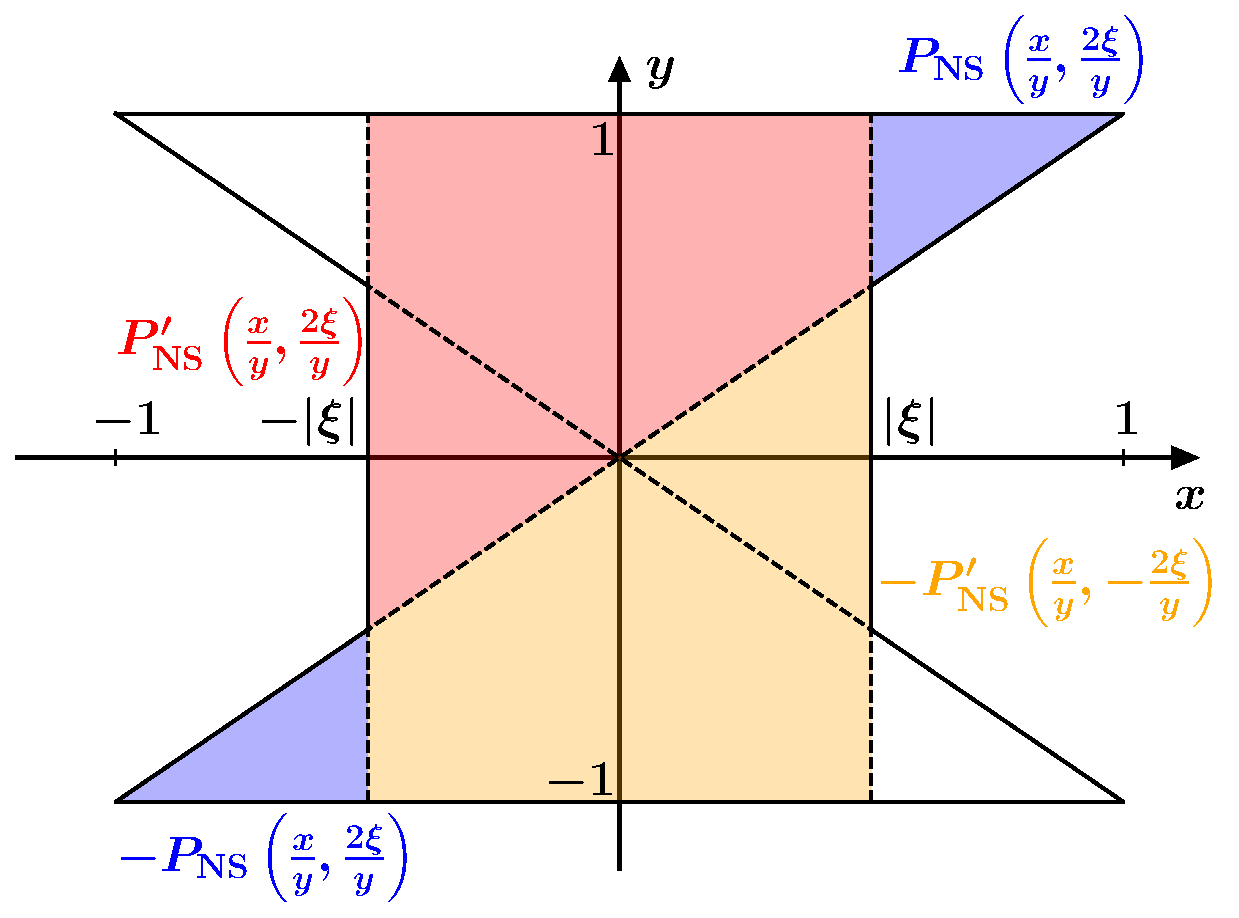
\includegraphics[width=0.7\textwidth]{plots/GPDIntDomain2.pdf}
    \caption{Support domain of the evolution kernel in Eq.~(\ref{eq:evkernelERBLgenxi}).\label{fig:GPDIntDomain2}}
  \end{centering}
\end{figure}
% We can now use Eq.~(\ref{eq:primevsnonprime}) to replace $P_{\rm NS}$
% with $P_{\rm NS}'$ which gives:
% \begin{equation}
% \begin{array}{rcl}
% \displaystyle \frac{1}{\xi}\mathbb{V}_{\rm NS}^{(0)}\left(\frac{x}{\xi}, \frac{y}{\xi}\right) &=& \displaystyle
% \frac{2}{y}\left[\theta(x-\xi) \theta(y-x)+\theta(\xi-x)\theta(\xi+x)\theta(y-x)-\theta(-x-\xi)
%                                               \theta(x-y)\right]P_{\rm NS}'\left(\frac{x}{y},\frac{2\xi}{y}\right)\\
% \\
% &+&\displaystyle \left[x\rightarrow -x, y\rightarrow -y\right] \\
% \\
% %&-&\displaystyle \frac{2}{y}\left[\theta(-x-\xi)
% %                                              \theta(x-y)+\theta(\xi+x)\theta(\xi-x)\theta(x-y) -\theta(x-\xi) \theta(y-x)\right]P_{\rm NS}'\left(\frac{x}{y},-\frac{2\xi}{y}\right) \\
% %\\
% &+&\displaystyle \delta\left(y-x\right) 2C_F\left[\frac{3}{2}+\int_\xi^{x}\frac{dz}{z-x}+\int_{-\xi}^{x}\frac{dz}{z-x}\right]\,.
% \end{array}
% \end{equation}
As we will see below, in order to compute conformal moments one needs
to convolute the evolution kernel with some function integrating over
the $x$ variable. To do so, we use Eq.~(\ref{eq:primevsnonprime}) to
write $P_{\rm NS}$ in terms of $P_{\rm NS}'$ then, referring to
Fig.~\ref{fig:GPDIntDomain2}, we integrate over the blue, read, and
orange regions separately reducing the convolution to integrals
between $\xi$ and $y$ and $-\xi$ and $y$ that can the be
gathered. Given a well-behaved test function $f$, the final result
reads:
\begin{equation}
\begin{array}{rcl}
\displaystyle \int_{-1}^{1}\frac{dx}{\xi}\mathbb{V}_{\rm
  NS}^{(0)}\left(\frac{x}{\xi}, \frac{y}{\xi}\right)f(x) &=&
                                                             \displaystyle
                                                             2C_F\Bigg\{\frac{3}{2}f(y)+\int_\xi^y
                                                             dx\left[\frac1{C_F
                                                             y}P_{\rm
                                                             NS}'\left(\frac{x}{y},-\frac{2\xi}{y}\right)
                                                             f(x)-\frac{f(y)}{y-x}\right]\\
\\
&+&\displaystyle \int_{-\xi}^y dx\left[\frac1{C_F y}P_{\rm
                                                             NS}'\left(\frac{x}{y},\frac{2\xi}{y}\right)
                                                             f(x)-\frac{f(y)}{y-x}\right]\Bigg\}\,.
\end{array}
\label{eq:evkernelERBLgenxi2}
\end{equation}
Considering that:
\begin{equation}
\frac{1}{C_Fy}P_{\rm NS}'\left(\frac{x}{y},\frac{2\xi}{y}\right) = \frac{x-\xi}{2\xi(y+\xi)}+\frac{1}{y-x}\,,
\end{equation}
and thus:
\begin{equation}
\frac{1}{C_Fy}P_{\rm NS}'\left(\frac{x}{y},-\frac{2\xi}{y}\right) = -\frac{x+\xi}{2\xi(y-\xi)}+\frac{1}{y-x}\,,
\end{equation}
one finally has:
\begin{equation}
\begin{array}{rcl}
\displaystyle \int_{-1}^{1}\frac{dx}{\xi}\mathbb{V}_{\rm
  NS}^{(0)}\left(\frac{x}{\xi}, \frac{y}{\xi}\right)f(x) &=&
                                                             \displaystyle
                                                             2C_F\Bigg\{\frac{3}{2}f(y)-\frac12\int_\xi^y
                                                             dx\left[\frac{x+\xi}{\xi(y-\xi)}f(x)-2\frac{f(x)-f(y)}{y-x} \right]\\
\\
&+&\displaystyle \frac12\int_{-\xi}^y dx\left[\frac{x-\xi}{\xi(y+\xi)}f(x)+2\frac{f(x)-f(x)}{y-x}\right]\Bigg\}\,.
\end{array}
\label{eq:evkernelERBLgenxi1}
\end{equation}


% Assuming $\xi$ positive and different from zero ($\xi>0$), a simple
% change of variables produces:
% \begin{equation}
% \frac{d}{d\ln\mu^2} f^{-}(\xi x,\xi)=
% \frac{\alpha_s(\mu)}{4\pi}\int_{-1/\xi}^{1/\xi}dy\, \mathbb{V}_{\rm NS}^{(0)}\left(x,y\right) f^{-}(\xi y,\xi)\,,
% \end{equation}
% where the evolution kernel is given by:
% \begin{equation}
% \begin{array}{rcl}
% \mathbb{V}_{\rm NS}^{(0)}\left(x,y\right) &=& \displaystyle
% \frac{2}{y}\bigg\{\theta(x-1) \theta(y-x)P_{\rm
%                                               NS}\left(\frac{x}{y},\frac{2}{y}\right)-\theta(-x-1)
%                                               \theta(x-y)P_{\rm
%                                               NS}\left(\frac{x}{y},\frac{2}{y}\right)\\
% \\
% &+&\displaystyle \theta(1-x)\theta(x+1) \left[\theta(y-x)P_{\rm
%     NS}'\left(\frac{x}{y},\frac{2}{y}\right)-\theta(x-y)P_{\rm
%     NS}'\left(\frac{x}{y},-\frac{2}{y}\right)\right]\\
% \\
% &+&\displaystyle \delta\left(1-\frac{x}{y}\right) C_F\left[\frac{3}{2}+\int_1^{x}\frac{dz}{z-x}+\int_{-1}^{x}\frac{dz}{z-x}\right]\bigg\}\,.
% \end{array}
% \end{equation}
% Observing that:
% \begin{equation}
% \int_{\pm 1}^{x}\frac{dz}{z-x} = \theta(x-1) \int_{\pm
%   1}^{x}\frac{dz}{z-x} \mp \theta(1-x)\theta(x+1)\int_{-1}^{1}\frac{dz\theta(\pm z \mp x)}{z-x}-\theta(-x-1) \int^{\pm
%   1}_{x}\frac{dz}{z-x}
% \end{equation}
% the result can be recasted as:
% \begin{equation}\label{eq:ERBLkernel}
% \begin{array}{rcl}
% \mathbb{V}_{\rm NS}^{(0)}\left(x,y\right) &=& \displaystyle
%                                               \theta(1-x)\theta(x+1){V}_{\rm
%                                               NS}^{(0)}\left(x,y\right)\\
% \\
% &+&\displaystyle
%     \theta(x-1) 2C_F\left[\theta(y-x)\frac{x^2+y^2-2}{(y-x)(y^2-1)}+\delta(x-y)\left(2\int_{1}^{x}\frac{dz}{z-x}+\int_{-1}^{1}\frac{dz}{z-x}\right)\right]\\
% \\
% &-&\displaystyle
%     \theta(-x-1) 2C_F\left[\theta(x-y)\frac{x^2+y^2-2}{(y-x)(y^2-1)}+\delta(x-y)\left(2\int^{-1}_{x}\frac{dz}{z-x}+\int^{1}_{-1}\frac{dz}{z-x}\right)\right]\,,
% \end{array}
% \end{equation}
% where ${V}_{\rm NS}^{(0)}$ is given in Eq.~(\ref{eq:ERBLkernelxy}). We
% remind, however, that this form of the ERBL kernel is valid for
% $\xi>0$. The limit $\xi\rightarrow 0$ requires considering
% Eq.~(\ref{eq:evkernelERBLgenxi}).

\subsubsection{Conformal moments}

A relevant question is whether Eq.~(\ref{eq:evkernelERBLgenxi}) is
such that the so-called conformal moments of non-singlet GPDs (see
Eq.~(111) of Ref.~\cite{Diehl:2003ny}):
\begin{equation}
  \mathcal{C}_n^-(\xi) =
  \xi^{n}\int_{-1}^{1}dx\,C_n^{3/2}\left(\frac{x}{\xi}\right)f^{-}(x,\xi)\,,
\label{eq:conformalmoments}
\end{equation}
where $C_n^{3/2}$ are Gegenbauer polynomials, ``diagonalise'' the
leading-order evolution equation in Eq.~(\ref{eq:ERBLlikeeveq}). To
state it differently, we would like to check whether conformal moments
evolve multiplicatively. Multiplying Eq.~(\ref{eq:ERBLlikeeveq}) by
$\xi^{n}C_n^{3/2}\left(x/\xi\right)$ and integrating over $x$ between
$-1$ and 1, yields:
\begin{equation}
\frac{d \mathcal{C}_n^-(\xi)}{d\ln\mu^2} =
\frac{\alpha_s(\mu)}{4\pi}\xi^{n}\int_{-1}^1 dy
f^{-}(y,\xi)\int_{-1}^{1}\frac{dx}{\xi}\,C_n^{3/2}\left(\frac{x}{\xi}\right)
\mathbb{V}_{\rm NS}^{(0)}\left(\frac{x}{\xi},\frac{y}{\xi}\right) \,.
\label{eq:confmomprel}
\end{equation}
Therefore, the aim is to check whether the following equality holds:
\begin{equation}
  \int_{-1}^1\frac{dx}{\xi}\,C_n^{3/2}\left(\frac{x}{\xi}\right)
  \mathbb{V}_{\rm NS}^{(0)}\left(\frac{x}{\xi},\frac{y}{\xi}\right)
  =\mathcal{V}_{n}^{(0)}(\xi)C_n^{3/2}\left(\frac{y}{\xi}\right)\,,
\label{eq:confmomgpd}
\end{equation}
where $\mathcal{V}_{n}^{(0)}$ is a number that may generally depend on
$\xi$. If Eq.~(\ref{eq:confmomgpd}) held, Eq.~(\ref{eq:confmomprel})
would become:
\begin{equation}
  \frac{d \mathcal{C}_n^-(\xi)}{d\ln\mu^2}
  =\frac{\alpha_s(\mu)}{4\pi}\mathcal{V}_{n}^{(0)}(\xi)\mathcal{C}_n^-(\xi)\,,
\label{eq:confmom}
\end{equation}
that is to say that conformal moments evolve multiplicative exactly
like Mellin moments for forward distributions. As a matter of fact, up
to numerical factor, conformal moments do coincide with Mellin moments
in the limit $\xi\rightarrow 0$. This can be seen by observing that
the Gegenbauer polynomials admit the following expansion:
\begin{equation}
\xi^{n}C_n^{3/2}\left(\frac{x}{\xi}\right)=\frac{n+1}{2^{n+1}}\sum_{k=0}^n{n
\choose k}{n+2 \choose k+1}(x+\xi)^k (x-\xi)^{n-k}\,,
\end{equation}
that is such that:
\begin{equation}
\lim_{\xi\rightarrow 0}
\xi^{n}C_n^{3/2}\left(\frac{x}{\xi}\right)=
\frac{(2n+1)!}{2^n(n!)^2}x^{n}\,.
\label{eq:gegenlimit}
\end{equation}
Therefore, the conformal moments of the non-singlet distribution in
the forward limit become:
\begin{equation}
\lim_{\xi\rightarrow 0}\mathcal{C}_n^-(\xi) = \frac{(2n+1)!}{2^n(n!)^2}[1+(-1)^n]f^{-}(n+1)\,,
\end{equation}
where, with abuse of notation, we have defined the Mellin moments of
the forward distribution as:
\begin{equation}
f^{-}(n) = \lim_{\xi\rightarrow 0} \int_0^1dx\,x^{n-1}f^{-}(x,\xi)\,,
\end{equation}
that are known to diagonalise the DGLAP equation to all orders. Using
Eq.~(\ref{eq:gegenlimit}) and the fact that:
\begin{equation}
\lim_{\xi\rightarrow 0} \frac{1}{\xi}\mathbb{V}_{\rm NS}^{(0)}\left(\frac{x}{\xi},
  \frac{y}{\xi}\right) = \left[\theta(x)\theta(y-x)-\theta(-x)\theta(x-y)\right]\frac{1}{y} P_{\rm NS}^{(0)}\left(\frac{x}{y}\right)\,,
\end{equation}
where $P_{\rm NS}^{(0)}$ is the leading-order non-singlet DGLAP
splitting function, one finds:
\begin{equation}
 \lim_{\xi\rightarrow 0}
 \int_{-1}^1\frac{dx}{\xi}\,C_n^{3/2}\left(\frac{x}{\xi}\right)
 \mathbb{V}_{\rm NS}^{(0)}\left(\frac{x}{\xi},\frac{y}{\xi}\right) = \frac{(2n+1)!}{2^n(n!)^2}y^{n} P_{\rm NS}^{(0)}(n+1) =\left[\lim_{\xi\rightarrow 0}
\xi^{n}C_n^{3/2}\left(\frac{y}{\xi}\right)\right]P_{\rm NS}^{(0)}(n+1)\,,
\end{equation}
where, again with abuse of notation, the Mellin moments of the
splitting functions are given by (see, \textit{e.g.}, Eq.~(4.129) of
Ref.~\cite{Ellis:1991qj}):
\begin{equation}
P_{\rm NS}^{(0)}(n) = \int_{0}^{1}dx\,x^{n-1}P_{\rm NS}^{(0)}(x) = 2C_F\left[-\frac12+\frac{1}{n(n+1)}-2\sum_{k=2}^{n}\frac{1}{k}\right]\,.
\end{equation}
Finally, Eq.~(\ref{eq:confmom}) is fulfilled and the evolution kernel
can be directly read off:
\begin{equation}
 \lim_{\xi\rightarrow 0} \mathcal{V}_{n}^{(0)}(\xi) = P_{\rm
   NS}^{(0)}(n+1)=
 2C_F\left[-\frac12+\frac{1}{(n+1)(n+2)}-2\sum_{k=2}^{n+1}\frac{1}{k}\right]\,.
\label{eq:forwardlimitconfmom}
\end{equation}

On the other hand, it is well known that the one-loop ERBL kernel
$V_{\rm NS}^{(0)}$ obeys the relation:
\begin{equation}
  \int_{-1}^{1}dx\,C_n^{3/2}\left(x\right) V_{\rm
    NS}^{(0)}\left(x,y\right) =V_{n}^{(0)} C_n^{3/2}\left(y\right)\,.
\label{eq:confmomerbl}
\end{equation}
Evidently, $V_{n}^{(0)}$ is the evolution kernel in the
$\xi\rightarrow 1$ limit and its expression can be read off from
Eq.~(2.19) of Ref.~\cite{Lepage:1980fj} where, to match our notation,
we have to flip the sign and removed the $\beta$-function:
\begin{equation}
\lim_{\xi\rightarrow 1}\mathcal{V}_{n}(\xi)= V_{n}^{(0)}=2C_F\left[-\frac12+\frac{1}{(n+1)(n+2)}-2\sum_{k=2}^{n+1}\frac{1}{k}\right]=
 2C_F\left[\frac32-\frac{1}{n+1}-\frac{1}{n+2}-2\sum_{k=1}^{n}\frac{1}{k}\right]\,.
\label{eq:ERBLkernel}
\end{equation}
Remarkably, this is identical to
Eq.~(\ref{eq:forwardlimitconfmom}). This finally means that
Eq.~(\ref{eq:confmom}) is fulfilled in both the $\xi\rightarrow 0$ and
$\xi\rightarrow 1$ limits and that in these limits the evolution
kernels are equal. In other words, conformal moments of forward
distributions and distribution amplitudes at leading order evolve
multiplicatively with the same anomalous dimension. This suggests that
the kernels $\mathcal{V}_{n}$ may be constant in $\xi$ and equal to
Eq.~(\ref{eq:forwardlimitconfmom}).

To prove this we need to compute Eq.~(\ref{eq:confmomgpd}) for a
generic value of $\xi$. To do so, we use
Eq.~(\ref{eq:evkernelERBLgenxi1}) for $\mathbb{V}_{\rm NS}^{(0)}$
replacing $f(x)$ with $C_n^{3/2}\left(x/\xi\right)$:
\begin{equation}
\begin{array}{rcl}
  \displaystyle
  \int_{-1}^1\frac{dx}{\xi}\,C_n^{3/2}\left(\frac{x}{\xi}\right)
  \mathbb{V}_{\rm NS}^{(0)}\left(\frac{x}{\xi},\frac{y}{\xi}\right)&=&\displaystyle 2C_F \Bigg\{\frac{3}{2}C_n^{3/2}\left(\frac{y}{\xi}\right) \\
\\
&-&\displaystyle \frac12\int_{\xi}^{y}dx\left[\frac{x+\xi}{\xi(y-\xi)}C_n^{3/2}\left(\frac{x}{\xi}\right) -2\frac{C_n^{3/2}\left(x/\xi\right)-C_n^{3/2}\left(y/\xi\right)}{y-x}\right]\\
\\
&+&\displaystyle \frac12\int_{-\xi}^{y}dx\left[\frac{x-\xi}{\xi(y+\xi)}C_n^{3/2}\left(\frac{x}{\xi}\right)+2\frac{C_n^{3/2}\left(x/\xi\right)-C_n^{3/2}\left(y/\xi\right)}{y-x}\right]\Bigg\}\,.
\end{array}
\label{eq:GPDevkernelalaERBL}
\end{equation}
Of course, in the limits $\xi\rightarrow 0$ and $\xi\rightarrow 1$
this expression produces the Gegenbauer polynomials in the respective
limits times $V_n^{0}$. The calculation for \textit{all} $n$ and for a
generic value of $\xi$ is not straightforward. To start with, we
compute the integral above for $n=0$ where we expected to obtain zero
because $V^{(0)}=0$. Since $C_0^{\alpha}(z)=1$, the zero-th conformal
moment evaluates to:
\begin{equation}
\begin{array}{rcl}
\displaystyle
  \int_{-1}^1\frac{dx}{\xi}\,C_0^{3/2}\left(\frac{x}{\xi}\right)
  \mathbb{V}_{\rm NS}^{(0)}\left(\frac{x}{\xi},\frac{y}{\xi}\right)  &=& \displaystyle
  C_F\left[3 - \int_{\xi}^{y}dx \frac{x+\xi}{\xi(y-\xi)}
+\int_{-\xi}^{y}dx\frac{x-\xi}{\xi(y+\xi)}\right]\\
\\
&=& \displaystyle C_F\left[3 -\frac{y+\xi}{2\xi}-1+\frac{y-\xi}{2\xi}-1\right]=0\,,
\end{array}
\end{equation}
providing further evidence that indeed Gegenbauer polynomials do
diagonalise GPD leading-order evolution with evolution kernels
$\mathcal{V}_n^{(0)}(\xi)=V_n^{(0)}$ independent of $\xi$.

Now let us consider the case $n=1$. In the case the Gegenbauer
polynomial is:
\begin{equation}
C_1^{3/2}\left(\frac{x}{\xi}\right)=\frac{3x}{\xi}\,.
\end{equation}
Since:
\begin{equation}
V_1^{(0)} = -\frac{8C_F}{3}\,,
\end{equation}
we expect:
\begin{equation}
  \int_{-1}^1\frac{dx}{\xi}\,C_1^{3/2}\left(\frac{x}{\xi}\right)
  \mathbb{V}_{\rm NS}^{(0)}\left(\frac{x}{\xi},\frac{y}{\xi}\right) \mathop{=}^{?} -\frac{8C_F y}{\xi}\,.
\end{equation}
Using Eq.~(\ref{eq:GPDevkernelalaERBL}) with $n=1$, we find:
\begin{equation}
\begin{array}{rcl}
  \displaystyle
  \int_{-1}^1\frac{dx}{\xi}\,C_1^{3/2}\left(\frac{x}{\xi}\right)
  \mathbb{V}_{\rm
  NS}^{(0)}\left(\frac{x}{\xi},\frac{y}{\xi}\right)&=&\displaystyle
                                                       \frac{3C_F}{\xi}\left[3y
                                                       -\int_{\xi}^{y}dx\left[\frac{x(x+\xi)}{\xi(y-\xi)}
                                                       +2\right]+\int_{-\xi}^{y}dx\left[\frac{x(x-\xi)}{\xi(y+\xi)}-2\right]\right]\\
\\
&=&\displaystyle \frac{3C_F}{\xi}\left[3y-4y-\frac{5}{3}y\right] = -\frac{8C_Fy}{\xi}\,,
\end{array}
\end{equation}
as expected. We can now attempt a general proof. To do so, we define
$z=y/\xi$ and, using a the change of variable $v=x/\xi$ in the
integrals, rewrite the r.h.s. of Eq.~(\ref{eq:GPDevkernelalaERBL})
without the factor $2C_F$ as follows:
\begin{equation}
\begin{array}{rcl}
  \displaystyle
I &=&\displaystyle \frac{3}{2}C_n^{3/2}\left(z\right) - \frac12\int_{1}^{z}dv\left[\frac{v+1}{z-1}C_n^{3/2}\left(v\right) -2\frac{C_n^{3/2}\left(v\right)-C_n^{3/2}\left(z\right)}{z-v}\right]\\
\\
&+&\displaystyle \frac12\int_{-1}^{z}dv\left[\frac{v-1}{z+1}C_n^{3/2}\left(v\right)+2\frac{C_n^{3/2}\left(v\right)-C_n^{3/2}\left(z\right)}{z-v}\right]\,.
\end{array}
\label{eq:integralmoms}
\end{equation}
Now we use the fact that $C_n^{3/2}$ is indeed a polynomial of degree
$n$ whose expansion reads:
\begin{equation}
  C_n^{3/2}(x) = \sum_{k=0}^{\lfloor n/2 \rfloor} a_k^{(n)}x^{\ell}\,\quad\mbox{with}\quad  a_k^{(n)} =
(-1)^k2^{\ell}\frac{\Gamma(\ell+k+3/2)}{\Gamma(3/2)k!\ell!}\,,
\end{equation}
with $\ell = n-2k$, that allows us to write:
\begin{equation}
I= \frac{3}{2}C_n^{3/2}\left(z\right)-  \frac12\sum_{k=0}^{\lfloor n/2 \rfloor} a_k^{(n)}\left[\int_{1}^{z}dv\frac{v^{\ell+1}+v^{\ell}}{z-1}-\int_{-1}^{z}dv\frac{v^{\ell+1}-v^{\ell}}{z+1} +2 \int_{1}^{z}dv\frac{z^{\ell}-v^{\ell}}{z-v}+2 \int_{-1}^{z}dv\frac{z^{\ell}-v^{\ell}}{z-v}\right]\,.
\end{equation}
Now we can solve the integrals. The first 
integral gives:
\begin{equation}
\int_{1}^{z}dv\frac{v^{\ell+1}+v^{\ell}}{z-1} = \frac1{\ell+2}\frac{1-z^{\ell+2}}{1-z}+\frac1{\ell+1}\frac{1-z^{\ell+1}}{1-z}=\frac{1}{\ell+2}\sum_{j=0}^{\ell+1}z^{j}+\frac{1}{\ell+1}\sum_{j=0}^{\ell}z^{j}\,,
\end{equation}
and similarly the second:
\begin{equation}
\int_{-1}^{z}dv\frac{v^{\ell+1}-v^{\ell}}{z+1}=-\frac{(-1)^{\ell+2}}{\ell+2}\sum_{j=0}^{\ell+1}(-z)^{j}+\frac{(-1)^{\ell+1}}{\ell+1}\sum_{j=0}^{\ell}(-z)^{j}\,,
\end{equation}
where we have used the geometric series:
\begin{equation}
\sum_{j=0}^{n} v^{j}=\frac{1-v^{n+1}}{1-v}\,.
\end{equation}
Their combination evaluates to:
\begin{equation}
  \int_{1}^{z}dv\frac{v^{\ell+1}+v^{\ell}}{z-1}-\int_{-1}^{z}dv\frac{v^{\ell+1}-v^{\ell}}{z+1}
  = \left[\frac{1}{\ell+2}+\frac{1}{\ell+1} \right]\sum_{j=0}^{\ell}\left[1+(-1)^{\ell-j}\right]z^{j}\,.
\end{equation}
Notice that the $z^{\ell+1}$ term vanishes because the projector is
null for $j=\ell+1$. Now we turn to the third and fourth integrals in
Eq.~(\ref{eq:integralmoms}):
\begin{equation}
\int_{1}^{z}dv\frac{z^{\ell}-v^{\ell}}{z-v} =
z^{\ell-1}\int_{1}^{z}dv\frac{1-(v/z)^{\ell}}{1-v/z}=
\sum_{j=0}^{\ell-1}z^{\ell-j-1}\int_{1}^{z}dv\,v^j =
\sum_{j=0}^{\ell-1}\frac{z^{\ell}-z^{\ell-j-1}}{j+1} =-\sum_{j=0}^{\ell-1}\frac{z^{j}}{\ell-j}+z^{\ell}\sum_{j=1}^{\ell}\frac{1}{j}\,,
\end{equation}
and:
\begin{equation}
\int_{-1}^{z}dv\frac{z^{\ell}-v^{\ell}}{z-v} =-\sum_{j=0}^{\ell-1}\frac{(-1)^{\ell-j}z^{j}}{\ell-j}+z^{\ell}\sum_{j=1}^{\ell}\frac{1}{j}\,,
\end{equation}
so that their combination gives:
\begin{equation}
2\int_{1}^{z}dv\frac{z^{\ell}-v^{\ell}}{z-v}+ 2\int_{-1}^{z}dv\frac{z^{\ell}-v^{\ell}}{z-v}=-2\sum_{j=0}^{\ell-1}\frac{1+(-1)^{\ell-j}}{\ell-j} z^{j}+z^{\ell}\sum_{j=1}^{\ell}\frac{4}{j}\,.
\end{equation}
Putting everything together one finds:
\begin{equation}
\begin{array}{rcl}
  \displaystyle
  I &=&\displaystyle \frac{3}{2}C_n^{3/2}\left(z\right)\\
  \\
  &-&\displaystyle  \sum_{k=0}^{\lfloor n/2 \rfloor} a_k^{(n)}\left[\sum_{j=0}^{\ell-1}\left(\frac{1}{\ell+2}+\frac{1}{\ell+1} -\frac{2}{\ell-j}\right)\frac{1+(-1)^{\ell-j}}{2}z^{j} +\left(\frac{1}{\ell+2}+\frac{1}{\ell+1} +\sum_{j=0}^{\ell-1}\frac{2}{j+1}\right)z^{\ell}\right]\,.
\end{array}
\end{equation}
Now we exchange the sums over $k$ and the first sum over $j$ in the
second line of the equation above by using the following equality:
\begin{equation}
  \sum_{k=0}^{\lfloor n/2 \rfloor}
  \sum_{j=0}^{\ell-1}\dots=\sum_{k=0}^{\lfloor n/2 \rfloor}
  \sum_{j=0}^{n-2k-1}\dots = \sum_{j=0}^{n-1}\sum_{k=0}^{\lfloor \frac{n-j-1}2 \rfloor}\dots\,,
\end{equation}
finding:
\begin{equation}
\begin{array}{rcl}
  \displaystyle
  I &=&\displaystyle \frac{3}{2}C_n^{3/2}\left(z\right)\\
  \\
  &-&\displaystyle \sum_{j=0}^{n-1}z^{j} \frac{1+(-1)^{n-j}}{2}\sum_{k=0}^{\lfloor \frac{n-j-1}2 \rfloor} a_k^{(n)}\left(\frac{1}{n-2k+2}+\frac{1}{n-2k+1}
      -\frac{2}{n-2k-j}\right) \\
\\
&-&\displaystyle \sum_{k=0}^{\lfloor n/2 \rfloor} z^{\ell} a_k^{(n)}\left(\frac{1}{\ell+2}+\frac{1}{\ell+1} +\sum_{j=0}^{\ell-1}\frac{2}{j+1}\right)\,.
\end{array}
\end{equation}
where in the first line we have made explicit $\ell=n-2k$ and used the
equality:
\begin{equation}
\frac{1+(-1)^{\ell-j}}{2} = \frac{1+(-1)^{n-2k-j}}{2}=\frac{1+(-1)^{n-j}}{2}\,.
\end{equation}
This projector nullifies all the terms in the first series over $j$
for which $n-j$ is odd selecting only the even ones. Therefore we can
identify the combination $n-j$ with an even index, \textit{i.e.}
$n-j=2h$, and remove the projector. Replacing the summation index $k$
with $h$ and making explicit the index $\ell$
also in the second line gives:
\begin{equation}
\begin{array}{rcl}
  \displaystyle
  I &=&\displaystyle \frac{3}{2}C_n^{3/2}\left(z\right)\\
  \\
  &-&\displaystyle \sum_{h=0}^{\lfloor n/2 \rfloor}a_h^{(n)}z^{n-2h} \left[\frac{1}{n-2h+2}+\frac{1}{n-2h+1}+ 2\sum_{j=1}^{n-2h}\frac{1}{j}+\sum_{j=1}^{h} \frac{a_{h-j}^{(n)}}{a_h^{(n)}}\left(\frac{1}{n-2h+2j+2}+\frac{1}{n-2h+2j+1}-\frac1j\right)\right]\,.
\end{array}
\label{eq:almostthere}
\end{equation}
It turns out that the term in the square brackets is independent of
the summation index $h$ (this statement can be easily verified
numerically but an analytic proof looks very hard to achieve).
% To see this we take the difference between that coefficient computed
% in a generic $h$ and in $h=0$ that gives:
% \begin{equation}
% \begin{array}{rcl}
% \Delta &=&\displaystyle \frac{2h}{(n+2)(n-2h+2)}+\frac{2h}{(n+1)(n-2h+1)}-
%            2\sum_{j=n-2h+1}^{n}\frac{1}{j}\\
% \\
% &+&\displaystyle \sum_{j=1}^{h}
%            \frac{a_{h-j}^{(n)}}{a_h^{(n)}}\left(\frac{1}{n-2h+2j+2}+\frac{1}{n-2h+2j+1}-\frac1j\right)
% \end{array}
% \end{equation}
% Now we use the following identity for the coefficient of the
% Gegenbauer polynomial expansion:
% \begin{equation}
% \frac{a_{h-1}^{(n)}}{a_{h}^{(n)}} =1-\frac{(n+2)(n+1)}{(n-2h+2)(n-2h+1)}=I_h^{(n)}\,,
% \end{equation}
% that implies:
% \begin{equation}
% a_{h-j}^{(n)} =a_{h}^{(n)} \prod_{p=0}^{j-1}I_{h-p}^{(n)}\,,
% \end{equation}
% and that allows us to write:
% \begin{equation}
% \begin{array}{rcl}
% \Delta &=&\displaystyle \frac{2h}{(n+2)(n-2h+2)}+\frac{2h}{(n+1)(n-2h+1)}-
%            2\sum_{j=n-2h+1}^{n}\frac{1}{j}\\
% \\
% &+&\displaystyle \sum_{j=1}^{h}
%            \prod_{p=0}^{j-1}I_{h-p}^{(n)}\left(\frac{1}{n-2h+2j+2}+\frac{1}{n-2h+2j+1}-\frac1j\right)
% \end{array}
% \end{equation}
%
%
% \newpage
% Or we take the different between $h$ and $h+1$:
% \begin{equation}
% \begin{array}{rcl}
%   \displaystyle
%   \Delta &=&   \displaystyle\left[\frac{1}{n-2h+2}+\frac{1}{n-2h+1}+ \frac{1}{n-2h}+\frac{1}{n-2h-1}+\sum_{j=1}^{h} \frac{a_{h-j}^{(n)}}{a_h^{(n)}}\left(\frac{1}{n-2h+2j+2}+\frac{1}{n-2h+2j+1}-\frac1j\right)
%       \right]\\
% \\
% &-&\displaystyle\left[\sum_{j=1}^{h} \frac{a_{h-j}^{(n)}}{a_{h+1}^{(n)}}\left(\frac{1}{n-2h+2j+2}+\frac{1}{n-2h+2j+1}-\frac1{j+1}\right)+\frac{a_{h}^{(n)}}{a_{h+1}^{(n)}}\left(\frac{1}{n-2h+2}+\frac{1}{n-2h+1}-1\right)
%       \right]
% \end{array}
% \end{equation}
% Now we use the following identity for the coefficient of the
% Gegenbauer polynomial expansion:
% \begin{equation}
% \frac{a_{h}^{(n)}}{a_{h+1}^{(n)}} =1-\frac{(n+1)(n+2)}{(n-2h)(n-2h-1)}\,,
% \end{equation}
% so that:
% \begin{equation}
% \begin{array}{rcl}
%   \displaystyle
%   \Delta &=&   \displaystyle\left[\frac{1}{n-2h}+\frac{1}{n-2h-1}+1-\sum_{j=1}^{h} \frac{a_{h-j}^{(n)}}{a_h^{(n)}}\frac1{j(j+1)}
%       \right]\\
% \\
% &+&\displaystyle\frac{(n+1)(n+2)}{(n-2h)(n-2h-1)}\left[\frac{1}{n-2h+2}+\frac{1}{n-2h+1}-1+\sum_{j=1}^{h} \frac{a_{h-j}^{(n)}}{a_{h}^{(n)}}\left(\frac{1}{n-2h+2j+2}+\frac{1}{n-2h+2j+1}-\frac1{j+1}\right)
%       \right]\,.
% \end{array}
% \end{equation}
% Now we define:
% \begin{equation}
% \Delta' = \frac{(n-2h)(n-2h-1)}{(n+1)(n+2)}\Delta\,,
% \end{equation}
% such that:
% \begin{equation}
% \begin{array}{rcl}
%   \displaystyle
%   \Delta' &=&   \displaystyle\frac{(n-2h)(n-2h-1)}{(n+1)(n+2)}\left[\frac{1}{n-2h}+\frac{1}{n-2h-1}+1-\sum_{j=1}^{h} \frac{a_{h-j}^{(n)}}{a_h^{(n)}}\frac1{j(j+1)}
%       \right]\\
% \\
% &+&\displaystyle\left[\frac{1}{n-2h+2}+\frac{1}{n-2h+1}-1+\sum_{j=1}^{h} \frac{a_{h-j}^{(n)}}{a_{h}^{(n)}}\left(\frac{1}{n-2h+2j+2}+\frac{1}{n-2h+2j+1}-\frac1{j+1}\right)
%       \right]\,.
% \end{array}
% \end{equation}
%
%This proves that the term in square brackets in
%Eq.~(\ref{eq:almostthere}) is constant in $h$.
Therefore, without loss of generality, we can set $h=0$ and pull it
out from the summation symbol, obtaining:
\begin{equation}\begin{array}{rcl}
  \displaystyle
  I &=&\displaystyle \frac{3}{2}C_n^{3/2}\left(z\right)- \left[\frac{1}{n+2}+\frac{1}{n+1}+
      2\sum_{j=1}^{n}\frac{1}{j}\right]\sum_{h=0}^{\lfloor n/2
      \rfloor}a_h^{(n)}z^{n-2h}\\
\\
   &=&\displaystyle \left[\frac{3}{2}-\frac{1}{n+2}-\frac{1}{n+1}- 2\sum_{j=1}^{n}\frac{1}{j}\right]C_n^{3/2}\left(z\right)
\end{array}
\end{equation}
which finally proves the identity:
\begin{equation}
  \int_{-1}^1\frac{dx}{\xi}\,C_n^{3/2}\left(\frac{x}{\xi}\right)\mathbb{V}_{\rm NS}^{(0)}\left(\frac{x}{\xi},\frac{y}{\xi}\right)  = V_n^{(0)}C_n^{3/2}\left(\frac{y}{\xi}\right)\,,
\end{equation}
with $V_n^{(0)}$ given in Eq.~(\ref{eq:ERBLkernel}).

These calculations confirm that conformal moments evolve
multiplicatively as:
\begin{equation}
  \frac{d \mathcal{C}_n^-(\xi)}{d\ln\mu^2}
  =\frac{\alpha_s(\mu)}{4\pi}{V}_{n}^{(0)}\mathcal{C}_n^-(\xi)\,.
\end{equation}
The solution to this equation is simply:
\begin{equation}
\mathcal{C}_n^-(\xi,\mu)
=\exp\left[\frac{V_{n}^{(0)}}{4\pi}\int_{\mu_0}^\mu
  d\ln\mu^2\alpha_s(\mu)\right]\mathcal{C}_n^-(\xi,\mu_0)\,,
\label{eq:ConfMomentsSolution}
\end{equation}
in which remarkably the evolution kernel does not depend on
$\xi$. This in turn means that the $\xi$ dependence of conformal
moments is entirely encoded in the initial scale moments and that
evolution leave it unchanged.

The question that remains to be answered is whether the knowledge of
the conformal moments of a GPD is enough to reconstruct its $x$
dependence.

\subsubsection{On the expansion of GPDs in terms of Gegenbauer
  polynomials}

In the previous section, we have shown that the conformal moments of a
non-singlet GPD, defined as in Eq.~(\ref{eq:conformalmoments}), evolve
multiplicatively at LO according to
Eq.~(\ref{eq:ConfMomentsSolution}). The question that remains to be
answered is whether it is possible to reconstruct any non-singlet GPD
by knowing all its conformal moments. In order to do so, one should be
able to expand any given GPD $f^{-}$ in terms of conformal moments:
\begin{equation}
f^{-}(x,\xi,\mu) = \sum_{m=0}^{\infty}
\mathcal{C}_m^-(\xi,\mu)f_m(x,\xi)\,,
\label{eq:GPDexpansion}
\end{equation}
where $f_n$ is some set of functions. In this way, the evolution of
$f^{-}$ would simply amount to evolving the single conformal moments
$\mathcal{C}_m^-$ using Eq.~(\ref{eq:ConfMomentsSolution}). However,
in order for Eq.~(\ref{eq:GPDexpansion}) to be true the set of
functions $f_n$ must obey the relation:
\begin{equation}
  \xi^{n}\int_{-1}^{1}dx\,C_n^{3/2}\left(\frac{x}{\xi}\right)
  f_m(x,\xi)=  \xi^{n-1}\int_{-1/\xi}^{1/\xi}dz\,C_n^{3/2}\left(z\right)
  f_m(\xi z,\xi)=\delta_{mn}\,.
\label{eq:orthogonality}
\end{equation}
For $\xi=1$, as is the case for the ERBL evolution equation of DAs,
one could exploit the orthogonality of Gegenbauer polynomials in the
interval $[-1:1]$ and would have that:
\begin{equation}
f_m(x,1) = \frac{2 m!(m+3/2)[\Gamma(3/2)]^2}{\pi\Gamma(m+3)}(1-x^2)C_m^{3/2}(x)\,,
\end{equation}
that exactly verifies Eq.~(\ref{eq:orthogonality}) for $\xi=1$. This
allows one to expand DAs in terms of Gegenbauer polynomials and
compute the evolution by evolving the single conformal
moments. However, for $\xi < 1$ Eq.~(\ref{eq:orthogonality}) requires
integrating the Gegenbauer polynomials outside the region $[-1:1]$
thus preventing the use of orthogonality. To overcome this problem, one
could define:
\begin{equation}
f_m(x,\xi) = \xi^{1-n}\theta(x + \xi) \theta(\xi-x) \frac{2 m!(m+3/2)[\Gamma(3/2)]^2}{\pi\Gamma(m+3)}\left(1-\frac{x^2}{\xi^2}\right)C_m^{3/2}\left(\frac{x}{\xi}\right)\,,
\end{equation}
that indeed satisfies Eq.~(\ref{eq:orthogonality}) but at the price of
introducing $\theta$-functions that require $f^-$ to be zero outside
the ERBL region, \textit{i.e.} for $x>\xi$ and $x<-\xi$. In other
words, in order for the expansion in Eq.~(\ref{eq:GPDexpansion}) to be
possible, one needs to require that:
\begin{equation}
f^{-}(x,\xi,\mu) = 0\quad\mbox{for}\quad x>\xi\quad\mbox{and}\quad x<-\xi\,,
\end{equation}
that is clearly not acceptable for a GPD. However, in
Ref.~\cite{Mueller:2005ed} one reads: ``[\dots] the restricted support
property of each individual term does not imply that the GPD vanishes
in the outer region [$x>\xi$ or $x<-\xi$]. Rather one should
understand this expansion [Eq.~(\ref{eq:GPDexpansion})] as an
ill-convergent sum of distributions (in the mathematical sense) that
yields a result which is non-zero in the outer region.'' Indeed, the
authors of Ref.~\cite{Mueller:2005ed} managed to find a way to make
Eq.~(\ref{eq:GPDexpansion}) different from zero for $x>\xi$ or
$x<-\xi$. This needs to be understood.

\subsubsection{Sum rules}\label{eq:sumruleNS}

A question arises: does the fact that the GPD anomalous dimension
(\textit{cfr.}  Eq.~(\ref{eq:nonzeroplusGPD})) does not admit a fully
$+$-prescribed form violate any conservation law? To answer this
question, we notice that the fact that the non-singlet DGLAP anomalous
dimension integrates to zero (see Eq.~(\ref{eq:dglapsplitting})), and
thus admits a $+$-prescribed form, derives from the conservation of
the total number of quarks minus anti-quarks (valence sum rule):
\begin{equation}
\int_0^1dx\, f^-(x,0) = \mbox{constant}\,.
\label{eq:valsumrulef}
\end{equation}
Taking the derivative of this equation w.r.t. $\ln\mu^2$ and using the
DGLAP equation gives:
\begin{equation}
\begin{array}{rcl}
0&=&\displaystyle\int_0^1dx\int_x^1\frac{dy}{y}
     \mathcal{P}_1^-(y,0)f^-\left(\frac{x}{y},0\right) =
     \int_0^1dy\,
     \mathcal{P}_1^-(y,0)\int_0^y\frac{dx}{y}\,f^-\left(\frac{x}{y},0\right)\\
\\
&=&\displaystyle \int_0^1dy\,
     \mathcal{P}_1^-(y,0)\int_0^1dz\,f^-\left(z,0\right) =
    \mbox{constant}\times\int_0^1dy\,\mathcal{P}_1^-(y,0)\quad\Leftrightarrow
    \quad \int_0^1dy\,\mathcal{P}_1^-(y,0) = 0\,.
\end{array}
\label{eq:valsumrule}
\end{equation}
This clearly justifies the requirement for $\mathcal{P}_1^-(y,0)$ to
be fully $+$-prescribed.

One may try to apply the same argument to GPDs. In this case the
valence sum rule generalises in:
\begin{equation}
\int_0^1 dx\,f^-(x,\xi) = F\,,
\label{eq:sumrule}
\end{equation}
where $F$ is independent of $\mu$ and $\xi$ but may (and does) depend
on the momentum transfer $t$. $F$ is usually referred to as form
factor. One should now take the derivative w.r.t. $\ln\mu^2$ and use
Eq.~(\ref{eq:jitot}) but in doing this one needs to take into account
that $\kappa=\xi/x$:
\begin{equation}
\begin{array}{rcl}
  0&=&\displaystyle \int_0^1
       dx\int_0^1\frac{dy}{y}\left[\theta(y-x)\mathcal{P}_1^{-,(0)}\left(\frac{x}{y},\frac{\xi}{x}\right)+\theta(\xi-x)
       \mathcal{P}_2^{-,(0)}\left(\frac{x}{y},\frac{\xi}{x}\right)\right]f^-\left(y,\xi\right)\\
\\
&=&\displaystyle \int_0^1 dy\,f^-\left(y,\xi\right) \left[\int_0^y\frac{dx}{y}\,\mathcal{P}_1^{-,(0)}\left(\frac{x}{y},\frac{\xi}{x}\right)+
       \int_0^\xi \frac{dx}{y}\, \mathcal{P}_2^{-,(0)}\left(\frac{x}{y},\frac{\xi}{x}\right)\right]\\
\\
&=&\displaystyle \int_0^1 dy\,f^-\left(y,\xi\right) \left[\int_0^1dz\,\mathcal{P}_1^{-,(0)}\left(z,\frac{\xi}{yz}\right)+
       \int_0^{\xi/y} dz\, \mathcal{P}_2^{-,(0)}\left(z,\frac{\xi}{yz}\right)\right]\,,
\end{array}
\end{equation}
In order for this relation to be identically true, it is necessary
that:
\begin{equation}
  \int_0^1dz\,\mathcal{P}_1^{-,(0)}\left(z,\frac{\xi}{yz}\right)+
  \int_0^{\xi/y} dz\,
  \mathcal{P}_2^{-,(0)}\left(z,\frac{\xi}{yz}\right)=0\,.
\label{eq:valsumruleGPD}
\end{equation}
Notice that for $\xi\rightarrow 0$, the equality above reduces to
Eq.~(\ref{eq:valsumrule}). It is interesting to verify
Eq.~(\ref{eq:valsumruleGPD}) plugging in the explicit expressions for
$\mathcal{P}_1^{-,(0)}$, Eq.~(\ref{eq:p1minus0}), and
$\mathcal{P}_2^{-,(0)}$, Eq.~(\ref{eq:p2minus0}). One finds:
\begin{equation}
  \int_0^1dz\,\mathcal{P}_1^{-,(0)}\left(z,\frac{\xi}{yz}\right)=2C_F\left[-\frac{3}{2}\frac{\xi^2}{\xi^2-y^2}-\ln\left(\left|1-\frac{\xi^2}{y^2}\right|\right)\right]\,,
\end{equation}
that correctly tends to zero as $\xi\rightarrow 0$, and:
\begin{equation}
  \int_0^{\xi/y} dz\, \mathcal{P}_2^{-,(0)}\left(z,\frac{\xi}{yz}\right)=2C_F\left[\frac{3}{2}\frac{\xi^2}{\xi^2-y^2}+\ln\left(\left|1-\frac{\xi^2}{y^2}\right|\right)\right]\,,
\end{equation}
such that Eq.~(\ref{eq:valsumruleGPD}) is fulfilled. Despite
Eq.~(\ref{eq:valsumruleGPD}) has been explicitly proved at one-loop,
the same relation must hold order by order in perturbation theory.

It is important to notice that the constraint on the non-singlet GPD
anomalous dimensions deriving from the valence sum rule, and resulting
in Eq.~(\ref{eq:valsumruleGPD}), does not take the form of a
$+$-prescription, Eq.~(\ref{eq:pludistributionn}). A further proof can
be given by considering the non-singlet GPD evolution equation given
in Eq.~(\ref{eq:eveq}) (see also Eq.~(99) of
Ref.~\cite{Diehl:2003ny}). The independence of the form factor from
$\mu$ immediately leads to:
\begin{equation}
\int_{-1}^1dx'
f(x',\xi)\int_{-1}^1dx\left[\hat{V}_{\rm NS}\left(\frac{x}{\xi},\frac{x'}{\xi}\right)\right]_+ = 0\,,
\end{equation}
where $\hat{V}_{\rm NS}$ is nothing but $V _{\rm NS}$ stripped of the
supposedly global $+$-prescription. Assuming $\xi$ positive and
different from zero ($\xi>0$), a simple change of variables gives:
\begin{equation}
  \int_{-1/\xi}^{1/\xi}dy'
  f(\xi y',\xi)\int_{-1/\xi}^{1/\xi}dy\left[\hat{V}_{\rm NS}\left(y,y'\right)\right]_+ = 0\,.
\end{equation}
Given the fact that the bounds of the inner integral are not $-1$ and
$1$, the effect of the $+$-prescription as given in
Eq.~(\ref{eq:pludistributionn}) cannot give zero. This prevents the
above equation to be identically fulfilled violating polynomiality of
GPDs. We can thus conclude that $V _{\rm NS}$ \textit{cannot} be
written as a fully $+$-prescribed function.

\subsection{The singlet sector}

Having ascertained that the evolution equation from
Ref.~\cite{Ji:1996nm} is well-behaved for the non-singlet distribution
$f^-$, we move on to consider the singlet $f_{\rm S}$ and gluon
$f_{\rm G}$ distributions. As in the standard DGLAP evolution
equation, singlet and gluon GPDs couple under evolution. Defining
$f^+$ as the column vector of singlet and gluon GPDs, the
corresponding anomalous dimension $\mathcal{P}^+$ is a matrix in
flavour space:
\begin{equation}
  \mathcal{P}^+=\begin{pmatrix}
    \mathcal{P}_{\rm SS}& \mathcal{P}_{\rm SG}\\
    \mathcal{P}_{\rm GS}& \mathcal{P}_{\rm GG}
\end{pmatrix}\,.
\label{eq:singmat}
\end{equation}
Following the same procedure discussed above for the non-singlet
distribution $f^-$, the one-loop evolution equation for $f^+$ reads:
\begin{equation}
  \mu^2\frac{d}{d\mu^2}f^+(x,\xi) =
  \frac{\alpha_s(\mu)}{4\pi}\int_x^\infty\frac{dy}{y}\mathcal{P}^{+,(0)}(y,\kappa)f^+\left(\frac{x}{y},\xi\right)\,,
\label{eq:jitotsing}
\end{equation}
with:
\begin{equation}
  \mathcal{P}^{+,(0)}(y,\kappa)= \theta(1-y)\mathcal{P}_1^{+,(0)}(y,\kappa)+\theta(\kappa-1)\mathcal{P}_2^{+,(0)}(y,\kappa)\,.
\end{equation}
The single splitting function matrices $\mathcal{P}_{1}$ and
$\mathcal{P}_2$ are derived from the expression Ref.~\cite{Ji:1996nm}
as:
\begin{equation}
\begin{array}{rcl}
\mathcal{P}_{1,\rm IJ}(y,\kappa) &=& 2P_{\rm IJ}(y,2\kappa y)= 2P_{\rm IJ}'(y,2\kappa y) +
                                2P_{\rm IJ}'(y,-2\kappa y)\,,\\
\\
\mathcal{P}_{2,\rm IJ}(y,\kappa) &=& - 2P_{\rm IJ}'(y,-2\kappa y) - 2P_{\rm IJ}'(-y,2\kappa y)\,,
\end{array}
\end{equation}
with $\rm I,J=S,G$. This leads to:
\begin{equation}
\left\{\begin{array}{rcl}
\mathcal{P}_{1,\rm SS}^{(0)}(y,\kappa) &=& \mathcal{P}_{1}^{-,(0)}(y,\kappa)\,,\\
\\
\mathcal{P}_{2,\rm SS}^{(0)}(y,\kappa) &=& \displaystyle
                                           2C_F\left[\frac{1+y+\kappa y+\kappa^3y^2}{\kappa(1+y)(1-\kappa^2y^2)}-\left(\frac{1}{1-y}\right)_{++}\right]\,,
\end{array}\right.
\end{equation}

\begin{equation}
\left\{\begin{array}{rcl}
\mathcal{P}_{1,\rm SG}^{(0)}(y,\kappa) &=& \displaystyle 4n_f T_R\left[\frac{y^2+(1-y)^2-\kappa^2y^2}{(1-\kappa^2y^2)^2}\right]\,,\\
\\
\mathcal{P}_{2,\rm SG}^{(0)}(y,\kappa) &=& \displaystyle 4n_f T_R(1-\kappa)\left[\frac{1-\kappa(\kappa+2)y^2}{\kappa(1-\kappa^2y^2)^2}\right]\,,
\end{array}\right.
\end{equation}

\begin{equation}
\left\{\begin{array}{rcl}
  \mathcal{P}_{1,\rm GS}^{(0)}(y,\kappa) &=& \displaystyle 2C_F\left[\frac{1+(1-y)^2-\kappa^2y^2}{y(1-\kappa^2y^2)}\right]\,,\\
  \\
  \mathcal{P}_{2,\rm GS}^{(0)}(y,\kappa) &=& \displaystyle-2C_F\frac{(1-\kappa)^2}{\kappa(1-\kappa^2 y^2)}\,,
\end{array}\right.
\end{equation}

\begin{equation}
  \left\{\begin{array}{rcl}
           \mathcal{P}_{1,\rm GG}^{(0)}(y,\kappa) &=& \displaystyle
                                                      4C_A\left[\left(\frac{1}{1-y}\right)_+-\frac{1+\kappa^2y}{1-\kappa^2y^2}+\frac{1}{(1-\kappa^2y^2)^2}\left(\frac{1-y}{y}+y(1-y)\right)\right]\\
           \\
                                                  &+&\displaystyle\delta(1-y)\left[\left(\frac{11C_A-4 n_f
                                                      T_R}{3}\right) -2C_A\ln(|1-\kappa^2|)\right]\,,\\
           \\
           % &=& \displaystyle
           %                                            4C_A\bigg[\left(\frac{1}{1-y}-\frac{\kappa^2y}{1-\kappa^2y^2}\right)_++\frac{1}{(1-\kappa^2y^2)^2}\left(\frac{1-y}{y}+y(1-y)-1+\kappa^2y^2\right)\\
           % \\
           %                                        &+&\displaystyle\delta(1-y)\left(\frac{11C_A-4 n_f T_R}{3}\right)\,,\\
           % \\
           \mathcal{P}_{2,\rm GG}^{(0)}(y,\kappa) &=& \displaystyle
                                                      2C_A\left[\frac{2(1-\kappa)(1+y^2)}{(1-\kappa^2y^2)^2}+\frac{\kappa^2(1+y)}{1-\kappa^2y^2}+\frac{1-\kappa^2}{1-\kappa^2y^2}\left(2-\frac{1}{\kappa}-\frac{1}{1+y}\right)
                                                      -\left(\frac{1}{1-y}\right)_{++}\right]
                                                      \,.
\end{array}\right.
\end{equation}
% Notice that in the second equality for $\mathcal{P}_{1,\rm GG}^{(0)}$
% we have used the integral:
% \begin{equation}
% \int_0^1dz\frac{\kappa^2z}{1-\kappa^2z^2} = -\frac{1}{2}\ln(|1-\kappa^2|)\,,
% \end{equation}
% to make the limit $\kappa\rightarrow 1$ explicitly convergent.

In all cases, the limit for $\kappa\rightarrow 0$ of $\mathcal{P}_1$
reproduces the one-loop DGLAP splitting functions. In addition, we
also notice that all $\mathcal{P}_2$'s are proportional to
$\kappa-1$. Along with the fact that all $\mathcal{P}_1$ are
well-behaved at $\kappa=1$:
\begin{equation}
\begin{array}{rcl}
\mathcal{P}_{1,\rm SS}^{(0)}(y,1) &=& \displaystyle 2C_F\left\{\left[\frac{1}{1-y}\right]_++\delta(1-y)\left[\frac32-\ln(2)\right]\right\}\,,\\
\\
\mathcal{P}_{1,\rm SG}^{(0)}(y,1) &=& \displaystyle \frac{4n_f T_R}{(1+y)^2}\,,\\
\\
  \mathcal{P}_{1,\rm GS}^{(0)}(y,1) &=& \displaystyle \frac{4C_F}{y(1+y)}\,,\\
  \\
  \mathcal{P}_{1,\rm GG}^{(0)}(y,1) &=& \displaystyle 4C_A\left[\left(\frac{1}{1-y^2}\right)_++\frac{1}{y(1+y)^2}\right]+\delta(1-y)\left(\frac{11C_A-4 n_f T_R }{3}\right)\,,
\end{array}
\end{equation}
this guarantees the continuity of GPDs across the point $x=\xi$.

Now, we explicitly verify that the pole at $y=|\kappa|^{-1}$ that
affects all splitting functions above cancels between
$\mathcal{P}_{1,\rm IJ}^{(0)}$ and $\mathcal{P}_{2,\rm IJ}^{(0)}$. We
find:
\begin{equation}
\lim_{y\rightarrow \kappa^{-1}} (1-\kappa^2y^2)
\mathcal{P}_{1,\rm SS}^{(0)}(y,\kappa) = - \lim_{y\rightarrow \kappa^{-1}} (1-\kappa^2y^2)
\mathcal{P}_{2,\rm SS}^{(0)}(y,\kappa) = -2C_F\frac{1+\kappa}{\kappa}\,,
\end{equation}
\begin{equation}
\lim_{y\rightarrow \kappa^{-1}} (1-\kappa^2y^2)^2
\mathcal{P}_{1,\rm SG}^{(0)}(y,\kappa) = - \lim_{y\rightarrow \kappa^{-1}} (1-\kappa^2y^2)^2
\mathcal{P}_{2,\rm SG}^{(0)}(y,\kappa) = \frac{8 n_f T_R(1-\kappa)}{\kappa}\,,
\end{equation}
\begin{equation}
\lim_{y\rightarrow \kappa^{-1}} (1-\kappa^2y^2)
\mathcal{P}_{1,\rm GS}^{(0)}(y,\kappa) = - \lim_{y\rightarrow \kappa^{-1}} (1-\kappa^2y^2)
\mathcal{P}_{2,\rm GS}^{(0)}(y,\kappa) = 2C_F\frac{(1-\kappa)^2}{\kappa}\,,
\end{equation}
\begin{equation}
\lim_{y\rightarrow \kappa^{-1}} (1-\kappa^2y^2)^2
\mathcal{P}_{1,\rm GG}^{(0)}(y,\kappa) = - \lim_{y\rightarrow \kappa^{-1}} (1-\kappa^2y^2)^2
\mathcal{P}_{2,\rm GG}^{(0)}(y,\kappa) = 4C_A\frac{(\kappa-1)(\kappa^2+1)}{\kappa^2}\,.
\end{equation}
These results confirm the cancellation of the pole at
$y=|\kappa|^{-1}$ in the integral in the r.h.s. of
Eq.~(\ref{eq:jitotsing}).

We now compute the ERBL limit by taking $\kappa\rightarrow 1/x$. To do
so, we use the ERBL-compliant form of the evolution equation:
\begin{equation}
  \mu^2\frac{d}{d\mu^2}\Phi^+(t) =
  \frac{\alpha_s(\mu)}{4\pi}\left[\int_{0}^1 du\,\overline{V}_{\rm
      S}^{(0)}(t,u) \Phi^+\left(u\right)\right] \,,
\label{eq:erblsing}
\end{equation}
with $\Phi^+(t) = f^+(x,1)$ and where $u$ and $t$ are defined in
Eq.~(\ref{eq:ERBLvariables}).  $\overline{V}_{\rm S}^{(0)}$ is a matrix
in flavour space with the same structure of $\mathcal{P}^+$ in
Eq.~(\ref{eq:singmat}), whose components can be written in terms of
the $P_{\rm IJ}'$ functions as follows:
\begin{equation}
\begin{array}{rcl}
V_{\rm SS}^{(0)}(t,u) &=&\displaystyle \theta(u-t)\left[\frac{2}{2u-1}P_{\rm
    SS}'\left(\frac{2t-1}{2u-1},\frac{2}{2u-1}\right)
                          \right]-C_F\delta\left(u-t\right)\int_{0}^1 du' \,\frac{\theta(u'-t)}{u'-t}\\
\\
&+&\displaystyle \theta(t-u)\left[-\frac{2}{2u-1}P_{\rm
    SS}'\left(\frac{2t-1}{2u-1},-\frac{2}{2u-1}\right)
                          \right]+C_F\delta\left(t-u\right)\int_{0}^{1}du'\,\frac{\theta(t-u')}{u'-t}\\
\\
&+&\displaystyle \frac32C_F\delta\left(u-t\right)\,, \\
\\
V_{\rm SG,GS}^{(0)}(t,u) &=&\displaystyle \theta(u-t)\left[\frac{2}{2u-1}P_{\rm
    SG,GS}'\left(\frac{2t-1}{2u-1},\frac{2}{2u-1}\right)
                          \right]\\
\\
&+&\displaystyle \theta(t-u)\left[-\frac{2}{2u-1}P_{\rm
    SG,GS}'\left(\frac{2t-1}{2u-1},-\frac{2}{2u-1}\right)
                          \right]\,,\\
\\
V_{\rm GG}^{(0)}(t,u) &=&\displaystyle \theta(u-t)\left[\frac{2}{2u-1}P_{\rm
    GG}'\left(\frac{2t-1}{2u-1},\frac{2}{2u-1}\right)
                          \right]-C_A\delta\left(u-t\right)\int_{0}^1 du' \,\frac{\theta(u'-t)}{u'-t}\\
\\
&+&\displaystyle \theta(t-u)\left[-\frac{2}{2u-1}P_{\rm
    GG}'\left(\frac{2t-1}{2u-1},-\frac{2}{2u-1}\right)
                          \right]+C_A\delta\left(t-u\right)\int_{0}^{1}du'\,\frac{\theta(t-u')}{u'-t}\\
\\
&+&\displaystyle \left(\frac{11C_A-4n_fT_R}{6}\right)\delta\left(u-t\right)\,.
\end{array}
\end{equation}
The explicit expressions read:
\begin{equation}
\begin{array}{rcl}
  V_{\rm SS}^{(0)}(t,u) &=&\displaystyle V_{\rm NS}^{(0)}(t,u)\,,\\
  \\
  V_{\rm SG}^{(0)}(t,u) &=&\displaystyle 2n_fT_R\left(\frac{2u-1}{2}\right) \left[\theta(u-t)\frac{t}{u}\left(\frac{2t-1}{u}-2\frac{1-t}{1-u}\right)-\theta(t-u)\left(\frac{1-t}{1-u}\right)\left(\frac{1-2t}{1-u}-2\frac{t}{u}\right)\right]\,,\\
  \\
  V_{\rm GS}^{(0)}(t,u) &=&\displaystyle C_F \left(\frac{2}{2t-1}\right)
                            \left[\theta(u-t)\left(2t-\frac{t^2}{u}\right)
                            -\theta(t-u) \left(2(1-t)-\frac{(1-t)^2}{1-u}\right)\right]\,,\\
  \\
  V_{\rm GG}^{(0)}(t,u) &=&\displaystyle \mbox{This is a little
                            convoluted\dots leave it for when I feel
                            like doing the calculation}\,.
\end{array}
\end{equation}

\subsubsection{Sum rules}\label{eq:sumruleSG}

As done above for the non-singlet splitting function, here we exploit
polynomiality and the GPDs and the momentum sum rule (MSR) of PDFs to check
the correctness of the singlet splitting functions. Before considering
GPDs, let us derive the constrain that the MSR has on the forward
splitting functions. The MSR states that the integral over the
longitudinal momentum fractions $x$ of the sum of all PDFs weighted by
$x$ represents the momentum fraction of all partons in the hadron and
thus is to be equal to one at all scales. The respective formula
reads:
\begin{equation}
\int_0^1dx\,x\left[f_{\rm S}(x,0)+f_{\rm G}(x,0)\right] = 1\,.
\end{equation}
We can now that the derivative w.r.t. $\ln\mu^2$ of both side of the
the equation above and, using the evolution equation we find:
\begin{equation}
\int_0^1dy\,y\left[\mathcal{P}_{1,\rm SS}(y,0)+\mathcal{P}_{1,\rm
    GS}(y,0)\right]\left[\int_0^1dz\,z f_{\rm S}(z,0)\right] + \int_0^1dy\,y\left[\mathcal{P}_{1,\rm SG}(y,0)+\mathcal{P}_{1,\rm
    GG}(y,0)\right]\left[\int_0^1dz\,z f_{\rm G}(z,0)\right] = 0\,.
\end{equation}
In order for this equation to be identically fulfilled for any pair of
distributions $f_{\rm S}$ and $f_{\rm G}$, one needs to have:
\begin{equation}
\begin{array}{rcl}
\displaystyle \int_0^1dy\,y\left[\mathcal{P}_{1,\rm SS}(y,0)+\mathcal{P}_{1,\rm
    GS}(y,0)\right] &=& 0 \,,\\
\\
 \displaystyle \int_0^1dy\,y\left[\mathcal{P}_{1,\rm SG}(y,0)+\mathcal{P}_{1,\rm
    GG}(y,0)\right] &=& 0\,.
\end{array}
\label{eq:MSRforward}
\end{equation}
Effectively, these equations are fulfilled by the DGLAP splitting
functions. We now wish to extend this argument to GPDs to find similar
relations for the splitting functions that apply to $\xi\neq 0$. To do
so, we use polynomiality of GPDs that for both singlet and gluon
reads:
\begin{equation}
\int_0^1dx\,xf_{\rm S(G)}(x,\xi) = A_{q(g)}+\xi^2 D_{q(g)}\,,
\end{equation}
where the coefficients $A$ and $D$ generally depend on the scale
$\mu$. However, it is well known that helicity-conserving ($H$) and
helicity-flip ($E$) GPDs have the same D-term but with opposite sign
such that, if we define $f_{\rm S(G)}$ as the sum of $H$ and $E$ the
$\xi^2$ term cancels and one is left with:
\begin{equation}
\int_0^1dx\,xf_{\rm S(G)}(x,\xi) = A_{q(g)}\,.
\end{equation}
Therefore the sum of $f_{\rm S}$ and $f_{\rm G}$ gives:
\begin{equation}
\int_0^1dx\,x\left[f_{\rm S}(x,\xi) + f_{\rm G}(x,\xi)\right]= A\,,
\end{equation}
with $A=A_q+A_g$. Importantly $A$ is an observable and thus
independent of the scale $\mu$. In addition, $H$ and $E$ obey the same
evolution equations. This allows us to take the derivative with
respect to $\ln\mu^2$ of both sides of the equation above and use the
evolution equations. Following the same steps as in
Sect.~\ref{eq:sumruleNS} leads to the following equalities:
\begin{equation}
\begin{array}{rcl}
\displaystyle 
  \int_0^1dz\,z\left[\mathcal{P}_{1,\rm SS}\left(z,\frac{\xi}{yz}\right)+\mathcal{P}_{1,\rm GS}\left(z,\frac{\xi}{yz}\right)\right]+
  \int_0^{\xi/y} dz\, z\left[\mathcal{P}_{2,\rm SS}\left(z,\frac{\xi}{yz}\right)+\mathcal{P}_{2,\rm GS}\left(z,\frac{\xi}{yz}\right)\right]&=&0\,,\\
\\
 \displaystyle \int_0^1dz\,z\left[\mathcal{P}_{1,\rm SG}\left(z,\frac{\xi}{yz}\right)+\mathcal{P}_{1,\rm GG}\left(z,\frac{\xi}{yz}\right)\right]+
  \int_0^{\xi/y} dz\, z\left[\mathcal{P}_{2,\rm SG}\left(z,\frac{\xi}{yz}\right)+\mathcal{P}_{2,\rm GG}\left(z,\frac{\xi}{yz}\right)\right]&=&0\,,
\end{array}
\label{eq:MSRoffforward}
\end{equation}
that hold at each single order in $\alpha_s$ and automatically reduce
to Eq.~(\ref{eq:MSRforward}) for $\xi\rightarrow 0$. It is now
important to verify that the one-loop splitting functions written
above obey these relations. We find:
\begin{equation}
\int_0^1dz\,z\left[\mathcal{P}^{(0)}_{1,\rm
    SS}\left(z,\frac{\xi}{yz}\right)+\mathcal{P}^{(0)}_{1,\rm
    GS}\left(z,\frac{\xi}{yz}\right)\right] = 2C_F\left[-\frac12\frac{\xi^2}{y^2-\xi^2}-\ln\left(\left|1-\frac{\xi^2}{y^2}\right|\right)\right]\,,
\end{equation}
and:
\begin{equation}
\int_0^{\xi/y} dz\, z\left[\mathcal{P}^{(0)}_{2,\rm SS}\left(z,\frac{\xi}{yz}\right)+\mathcal{P}^{(0)}_{2,\rm GS}\left(z,\frac{\xi}{yz}\right)\right]= 2C_F\left[\frac12\frac{\xi^2}{y^2-\xi^2}+\ln\left(\left|1-\frac{\xi^2}{y^2}\right|\right)\right]\,,
\end{equation}
that evidently cancel so that the first of
Eq.~(\ref{eq:MSRoffforward}) is satisfied. In addition, they both tend
to zero as $\xi\rightarrow 0$ as required by the first of
Eq.~(\ref{eq:MSRforward}). Then we find:
\begin{equation}
\begin{array}{rcl}
\displaystyle\int_0^1dz\,z\left[\mathcal{P}^{(0)}_{1,\rm
    SG}\left(z,\frac{\xi}{yz}\right)+\mathcal{P}^{(0)}_{1,\rm
    GG}\left(z,\frac{\xi}{yz}\right)\right] &=&\displaystyle
  \frac{y^2\xi^2}{3(y^2-\xi^2)^2}\left[C_A\left(\frac{11\xi^2}{y^2}-4\right)+2n_fT_R\left(1-\frac{2\xi^2}{y^2}\right)\right]\\
\\
&-&\displaystyle 2C_A\ln\left(\left|\frac{y^2-\xi^2}{y^2}\right|\right)\,,
\end{array}
\end{equation}
and:
\begin{equation}
\begin{array}{rcl}
\displaystyle \int_0^{\xi/y} dz\, z\left[\mathcal{P}^{(0)}_{2,\rm
  SG}\left(z,\frac{\xi}{yz}\right)+\mathcal{P}^{(0)}_{2,\rm
  GG}\left(z,\frac{\xi}{yz}\right)\right]&=& \displaystyle
                                             -\frac{y^2\xi^2}{3(y^2-\xi^2)^2}\left[C_A\left(\frac{11\xi^2}{y^2}-4\right)+2n_fT_R\left(1-\frac{2\xi^2}{y^2}\right)\right]\\
\\
&+&\displaystyle 2C_A\ln\left(\left|\frac{y^2-\xi^2}{y^2}\right|\right)\,,
\end{array}
\end{equation}
so that also the second of Eq.~(\ref{eq:MSRoffforward}) is
satisfied. Again, their limit for $\xi\rightarrow 0$ tends to zero
that is consistent with the second of Eq.~(\ref{eq:MSRforward}).

\subsubsection{Conformal moments}

In this section, we discuss the diagonalisation of the GPD evolution
equation for the single distributions in conformal space. More
specifically, we first write the evolution kernels in an ERBL-like
form and then compute the conformal moments using the appropriate
Gegenbauer polynomials showing that they are eigenfunctions of the
kernels.

Similarly to the non-singlet sector, the GPD evolution equation for
the vector of singlet distributions reads:
\begin{equation}
\frac{d}{d\ln\mu^2} f^{+}(x,\xi)=
\frac{\alpha_s(\mu)}{4\pi}\int_{-1}^1\frac{dy}{\xi} \mathbf{V}^{(0)}\left(\frac{x}{\xi},\frac{y}{\xi}\right) f^{+}(y,\xi)\,,
\label{eq:ERBLlikeeveq}
\end{equation}
where $\mathbf{V}^{(0)}$ is a two by two matrix with components:
\begin{equation}
\begin{array}{rcl}
\displaystyle \frac{1}{\xi}\mathbf{V}_{\rm IJ}^{(0)}\left(\frac{x}{\xi}, \frac{y}{\xi}\right) &=& \displaystyle
\frac{2}{y}\bigg\{\left[\theta(x-\xi) \theta(y-x)+\theta(\xi-x)\theta(x+\xi)\theta(y-x)-\theta(-x-\xi)
                                              \theta(x-y)\right]P_{\rm IJ}'\left(\frac{x}{y},\frac{2\xi}{y}\right)\\
\\
&+&\displaystyle \left[\theta(x-\xi) \theta(y-x)-\theta(\xi-x)\theta(x+\xi)\theta(x-y)-\theta(-x-\xi)
                                              \theta(x-y)\right]P_{\rm IJ}'\left(\frac{x}{y},-\frac{2\xi}{y}\right)\\
\\
&+&\displaystyle \delta_{\rm IJ}\delta\left(1-\frac{x}{y}\right)
    C_{\rm I}\left[K_{\rm I}+\int_\xi^{x}\frac{dz}{z-x}+\int_{-\xi}^{x}\frac{dz}{z-x}\right]\bigg\}\,,\quad
    {\rm I,J=S,G}\,,
\end{array}
\end{equation}
with $C_{\rm S} = C_F$ and $C_{\rm G} = C_A$ and:
\begin{equation}
K_{\rm S}=\frac{3}{2}\quad\mbox{and}\quad K_{\rm G} = \frac{11C_A-4n_fT_R}{6C_A}\,.
\end{equation}
The conformal moments of the singlet kernels can be found by
generalising Eq.~(\ref{eq:evkernelERBLgenxi2}):
\begin{equation}
\begin{array}{rcl}
\displaystyle \int_{-1}^{1}\frac{dx}{\xi}\mathbf{V}_{\rm
  IJ}^{(0)}\left(\frac{x}{\xi}, \frac{y}{\xi}\right)f(x) &=&
                                                             \displaystyle
                                                             2C_{\rm
                                                             I}\Bigg\{\delta_{\rm
                                                             IJ}K_{\rm
                                                             I}f(y)+\int_\xi^y
                                                             dx\left[\frac1{C_{\rm I}
                                                             y}P_{\rm
                                                             IJ}'\left(\frac{x}{y},-\frac{2\xi}{y}\right)
                                                             f(x)-\delta_{\rm
                                                             IJ}\frac{f(y)}{y-x}\right]\\
\\
&+&\displaystyle \int_{-\xi}^y dx\left[\frac1{C_{\rm I} y}P_{\rm
                                                             IJ}'\left(\frac{x}{y},\frac{2\xi}{y}\right)
                                                             f(x)-\delta_{\rm
                                                             IJ}\frac{f(y)}{y-x}\right]\Bigg\}\,,
\end{array}
\label{eq:ConfMomsSing}
\end{equation}
and replacing $f(x)$ with the appropriate Gegenbauer polynomial
computed in $x/\xi$. Since
$\mathbf{V}_{\rm SS}^{(0)}=\mathbb{V}_{\rm NS}^{(0)}$, the SS
component has $C_n^{3/2}(x/\xi)$ as eigenfunctions with eigenvalues
$V_{{\rm SS}, n}^{(0)} = V_n^{(0)}$ given in
Eq.~(\ref{eq:ERBLkernel}). The eigenvalues of the remaining kernels
are expected to be:
\begin{equation}
\begin{array}{rcl}
\displaystyle V_{{\rm SS}, n}^{(0)} &=&\displaystyle V_n^{(0)}\,,\\
\\
\displaystyle V_{{\rm SG}, n}^{(0)} &=&\displaystyle P_{\rm
                                        SG}^{(0)}(n+1)=2T_R\frac{4+3n+n^2}{(n+1)(n+2)(n+3)}\,,\\
\\
\displaystyle V_{{\rm GS}, n}^{(0)} &=&\displaystyle P_{\rm
                                        GS}^{(0)}(n+1)=2C_F\frac{4+3n+n^2}{n(n+1)(n+2)}\,,\\
\\
\displaystyle V_{{\rm GG}, n}^{(0)} &=&\displaystyle P_{\rm
                                        GG}^{(0)}(n+1)=2C_A\left[K_{\rm
                                        G}+\frac{1}{n(n+1)}+\frac{1}{(n+2)(n+3)}-\sum_{k=1}^{n+1}\frac1k\right]\,,
\end{array}
\end{equation}
However, we still need to determine the degree of the Gegenbauer
polynomials that provide eigenfunction to the kernles. To do so, we
replace $f(x)=C_1^{\alpha}(x)=2\alpha x$ in
Eq.~(\ref{eq:ConfMomsSing}) and determine the value of $\alpha$ by
requiring that the integral equals
$V_{{\rm SS}, 1}^{(0)}C_1^{\alpha}(x)$.  We start with the GS kernel:
\begin{equation}
\begin{array}{rcl}
\displaystyle \int_{-1}^{1}\frac{dx}{\xi}\mathbf{V}_{\rm
  GS}^{(0)}\left(\frac{x}{\xi},
  \frac{y}{\xi}\right)C_n^{\alpha}\left(\frac{x}{\xi}\right) &=&
                                                                 \displaystyle 
C_F\left[\int_{-1}^z\frac{dv}{v}\frac{(v+1)(2z-v+1)}{z+1}C_n^{\alpha}\left(\frac{x}{\xi}\right)-\int_1^z\frac{dv}{v}\frac{(v-1)(2z-v-1)}{z-1}C_n^{\alpha}\left(\frac{x}{\xi}\right)\right]\,,
\end{array}
\end{equation}
with $z = y/\xi$. For $n=1$ we get:
\begin{equation}
\displaystyle \int_{-1}^{1}\frac{dx}{\xi}\mathbf{V}_{\rm
  GS}^{(0)}\left(\frac{x}{\xi},
  \frac{y}{\xi}\right)C_1^{\alpha}\left(\frac{x}{\xi}\right) = C_F\frac{16}{3}\alpha
    z=V_{{\rm GS}, 1}^{(0)}C_1^{\alpha}(z)\quad \forall \alpha\,,
\end{equation}
so we get no information on $\alpha$ from the first
moment. For the third moment we find:
\begin{equation}
\begin{array}{rcl}
\displaystyle \int_{-1}^{1}\frac{dx}{\xi}\mathbf{V}_{\rm
  GS}^{(0)}\left(\frac{x}{\xi},
  \frac{y}{\xi}\right)C_3^{\alpha}\left(\frac{x}{\xi}\right)
  &=&\displaystyle \frac{11}{15}C_F\left[-2\alpha(\alpha+1) z
      \frac{116-2\alpha}{33}+\frac43\alpha(\alpha+1)(\alpha+2)z^3\right]
\end{array}
\end{equation}



For the SG component we find:
\begin{equation}
\int_{-1}^{1}\frac{dx}{\xi}\mathbf{V}_{\rm
 SG}^{(0)}\left(\frac{x}{\xi}, \frac{y}{\xi}\right)C_n^{3/2}\left(\frac{x}{\xi}\right) =
                                                            \frac{T_R\xi z^2}{z^2-1}\left[\int_{-1}^{z} d{v}(v-z)\left(1-\frac{2v}{z+1}\right)
                                                            C_n^{3/2}\left(v\right)-\int_1^{z}
                                                            d{v}(v-z)\left(1-\frac{2v}{z-1}\right)
                                                            C_n^{3/2}\left(v\right)\right]\,,
\end{equation}
with $x = y/\xi$




\newpage
\section{Compton form factor}

In this section, we discuss the numerical implementation of the
Compton form factors (CFFs) for double deeply-virtual Compton
scattering (DDVCS). The CFFs can be regarded as the GPD counterpart of
the deep-inelastic scattering (DIS) structure function. The relation
is easily established by observing that the diagrams necessary to
compute the DIS structure functions at a given order are exactly the
same diagrams of DDVCS in the forward limit with a cut on the final
state. It is well-known that cut and uncut digrams are related through
dispersion relation. Specifically, ($2\pi i$ times) a given cut
diagram with an external on-shell momentum $p$ is equal to the
discontinuity of the uncut diagram in the forward limit along the
branch cut on the real axis determined by $p^2\geq m^2$, where $m$ is
the rest mass of the external particle. For the CCF $\mathcal{H}$,
this translates into the following relation with the DIS structure
function $F_1$:(\footnote{An additional factor 2 is included by
  convention in the definition of $F_1$.})
\begin{equation}
\lim_{\xi\rightarrow 0}
\left[\mathcal{H}(x+i\varepsilon,\xi,t,Q)-\mathcal{H}(x-i\varepsilon,\xi,t,Q)\right]
= 4\pi i F_1(x,Q)\,.
\end{equation}
Analyticity of the amplitude implies that
$\mathcal{H}(x-i\varepsilon,\xi,t,Q) =
\mathcal{H}^*(x+i\varepsilon,\xi,t,Q)$ which finally gives:
\begin{equation}
  \frac{1}{2\pi} \lim_{\xi\rightarrow 0}
  \mbox{Im}\left[\mathcal{H}(x,\xi,t,Q)\right] = F_1(x,Q)\,.
\label{eq:opticalth}
\end{equation}
An analogous relation exists between the CFF $\widetilde{\mathcal{H}}$
and the polarised structure function $g_5$ as well as between the
longitudinal projections $\mathcal{H}_L$ and
$\widetilde{\mathcal{H}}_L$, and $F_L$ and $g_L$, respectively. These
relation can be used to check that coefficient functions for the CCFs
reproduce the well-know DIS coefficient functions in the forward
limit.

Factorisation for DDVCS allows one to write CFFs as convolution
between short-distance partonic cross sections (or coefficient
functions) and nucleon GPDs. For $\mathcal{H}$ factorisation reads:
\begin{equation}
  \mathcal{H}(x,\xi,t,Q) =
  \sum_{q}e_q^2\int_{-1}^{1}\frac{dy}{y}\left[C_q\left(\frac{x}{y},\frac{\xi}{x},Q\right)F_q(y,\xi,t,Q)+C_g\left(\frac{x}{y},\frac{\xi}{x},Q\right)F_g(y,\xi,t,Q)\right]
\label{eq:CCFfact}
\end{equation}
where $e_q^2$ is the electric charge of the flavour $q$(\footnote{We
  are assuming that $Q\ll M_Z$ so that weak corrections to the
  electroweak coupling can be neglected.}) with the sum running over
the \textit{active} flavours (and not over the anti-flavours). $F_q$
and $F_g$ are the quark $q$ and gluon GPDs, respectively, and $C_q$
and $C_g$ the respective coefficient functions that admit a
perturbative expansion in powers of $\alpha_s$:
\begin{equation}
C_q\left(y,\kappa,Q\right) =
\sum_{n=0}^{\infty}\left(\frac{\alpha_s(Q)}{4\pi}\right)^nC_q^{(n)}\left(y,\kappa\right)\quad\mbox{and}\quad
C_g\left(y,\kappa,Q\right) =
\sum_{n=1}^{\infty}\left(\frac{\alpha_s(Q)}{4\pi}\right)^nC_g^{(n)}\left(y,\kappa\right)\,.
\label{eq:cffalstructfuncERBL}
\end{equation}
Currently, corrections up to $n=2$ are known~\cite{Mankiewicz:1997bk,
  Ji:1998xh, Pire:2011st, Braun:2020yib}. For implementation purposes,
it is convenient to rewrite Eq.~(\ref{eq:CCFfact}) as follows:
\begin{equation}
\begin{array}{rcl}
  x\mathcal{H}(x,\xi,t,Q) &=&\displaystyle
                             \sum_{q}e_q^2\int_{x}^{\infty}dy\bigg[C_q\left(y,\kappa,Q\right) \frac{x}{y} F_q\left(\frac{x}{y},\xi,t,Q\right)
                             + C_q\left(y,-\kappa,Q\right) \frac{x}{y} F_{\overline{q}}\left(\frac{x}{y},\xi,t,Q\right)\\
  \\
                         &+& \displaystyle  \left[C_g\left(y,\kappa,Q\right)+C_g\left(y,-\kappa,Q\right)\right]\frac{x}{y} F_g\left(\frac{x}{y},\xi,t,Q\right)\bigg]\,,
\end{array}
\label{eq:cffalstructfunc}
\end{equation}
with $\kappa=\xi/x$ and where we have exploited the symmetries
$C_{q,g}\left(y,\kappa,Q\right)=C_{q,g}\left(-y,-\kappa,Q\right)$ and
$F_g(y,\xi,t,Q)=-F_g(-y,\xi,t,Q)$, and defined
$F_{\overline{q}}(y,\xi,t,Q)=-F_q(-y,\xi,t,Q)$.

At first order ($n=0$), only the quark channel contributes and the
respective coefficient function is:
\begin{equation}
  C_q^{(0)}\left(y,\kappa\right) = -\frac{1}{1-y+i\varepsilon}-\frac{1}{1+y-i\varepsilon}\,.
\end{equation}
In order to get rid of the $i\varepsilon$ that complicates the
implementation, we use the following identity:
\begin{equation}
\frac{1}{X \mp i\varepsilon} = {\rm PV}\frac{1}{X} \pm \pi
i\delta(X)\,
\label{eq:princval}
\end{equation}
where PV stands for principal value, so that:
\begin{equation}
  C_q^{(0)}\left(y,\kappa\right) = {\rm PV}\left[-\frac{1}{1- y}-\frac{1}{1+ y}\right] + \pi i\left[\delta(1-y) - \delta(1+y)\right]\,.
\end{equation}
Plugging this into Eq.~(\ref{eq:cffalstructfunc}), defining
$\overline{F}_q^{+}(y,\xi,t,Q) =
y(F_q(y,\xi,t,Q)+F_{\overline{q}}(y,\xi,t,Q))$, and understanding the
principal value gives:
\begin{equation}
\begin{array}{rcl}
  x\mathcal{H}^{\rm LO}(x,\xi,t,Q) &=&\displaystyle
                                       \sum_{q}e_q^2\int_{x}^{\infty}dy\left[-\left(\frac{1}{1-
                                       y}\right)_{++}-\frac{1}{1+ y}+\pi i\delta(1-y)\right]
                                       \overline{F}_q^{+}\left(\frac{x}{y},\xi,t,Q\right)\,,
\end{array}
\end{equation}
where we have also introduced the $++$-prescription defined in
Eq.~(\ref{eq:plusplusdist}) that makes the integrand finite over the
integration range making it numerically computable. It is intersting
to observe that applying Eq.~(\ref{eq:opticalth}) to the leading-order
CFF gives the expected result:
\begin{equation}
  \frac{1}{2\pi} \lim_{\xi\rightarrow 0} \mbox{Im}\left[x\mathcal{H}^{\rm
      LO}(x,\xi,t,Q)\right] = \frac12\sum_{q}e_q^2xf_q^{+}(x,Q) =
  xF_1^{\rm LO}(x,Q)\,,
\end{equation}
where $f_q^+$ are the forward PDFs. The particular structure of
Eq.~(\ref{eq:cffalstructfunc}) allows one to relate real and imaginary
part of the CFF by observing that:
\begin{equation}
\begin{array}{rcl}
\displaystyle \mbox{Im}\left[x\mathcal{H}^{\rm
      LO}(x,\xi,t,Q)\right] &=& \displaystyle  \pi \sum_{q}e_q^2
  \overline{F}_q^{+}\left(x,\xi,t,Q\right)\,,\\
\\
\displaystyle \mbox{Re}\left[x\mathcal{H}^{\rm
      LO}(x,\xi,t,Q)\right] &=& \displaystyle \int_{x}^{\infty}dy\left[-\left(\frac{1}{1-
                                       y}\right)_{++}-\frac{1}{1+ y}\right]
                                       \sum_{q}e_q^2\overline{F}_q^{+}\left(\frac{x}{y},\xi,t,Q\right)\,.
\end{array}
\end{equation}
Therefore, one can plug the first into the second obtaining:
\begin{equation}
\mbox{Re}\left[x\mathcal{H}^{\rm
      LO}(x,\xi,t,Q)\right] =\frac{1}{\pi}\int_{x}^{\infty}dy\left[-\left(\frac{1}{1-
                                       y}\right)_{++}-\frac{1}{1+ y}\right]\mbox{Im}\left[x\mathcal{H}^{\rm
      LO}\left(\frac{x}{y},\xi,t,Q\right)\right]\,.
\end{equation}
This relation, often referred to as \textit{dispersion} relation, is
strictly valid only at leading order and is a useful tool when
extracting GPDs (or CFFs) from experimental data.

We can now move to consider the $\mathcal{O}(\alpha_s)$ corrections to
the CCF $\mathcal{H}$. At this order, both the quark and the gluon
channels contribute. We take the analytic expressions from
Ref.~\cite{Pire:2011st}. For the quark channel we use the finite part
of Eq.~(46) and for the gluon the finite part of Eq.~(47). Since we
are assuming $x_{\rm B}>0$ ($=x$ in our notation), we need to take
$Q^2>0$. In addition, our definition of coefficient functions in
Eq.~(\ref{eq:cffalstructfuncERBL}) is such that the expressions of
Ref.~\cite{Pire:2011st} have to be identified with
$(1/x)C_{q,g}^{(1)}(x_{\rm B}/x,\xi/x_{\rm B})$. This gives:
\begin{equation}
\begin{array}{rcl}
C_{q}^{(1)}(y,\kappa) &=& \displaystyle -\frac{C_F}{1-y+i\varepsilon}\bigg\{ -
                          9 +
                          3\frac{1-\kappa^2y^2-2y}{1-\kappa^2y^2}\ln\left(-\frac{1-y}{y}-i\varepsilon\right)+\frac{1+y^2 -2\kappa^2y^2}{1-\kappa^2y^2} \ln^2\left(-\frac{1-y}{y}-i\varepsilon\right)\\
\\
&+&\displaystyle 6\frac{\kappa(1-\kappa)y^2}{1-\kappa^2
    y^2}\ln(1-\kappa-i\varepsilon)+
\frac{(1-\kappa)(1-y-2\kappa^2 y^2)}{\kappa(1-\kappa^2
    y^2)}\ln^2(1-\kappa-i\varepsilon)\bigg\}\\
\\
&+& (y\rightarrow -y, \kappa\rightarrow -\kappa) \,,\\
\\
C_{g}^{(1)}(y,\kappa) &=& \displaystyle T_R \left(-\frac{1}{1-y+i\varepsilon}-\frac{1}{1+y-i\varepsilon}\right)\\
\\
&\times&\displaystyle \bigg\{ 
                          2\ln\left(-\frac{1-y}{y}-i\varepsilon\right)
                          +\frac{1-2y+2y^2-\kappa^2 y^2}{1-\kappa^2
                          y^2}\ln^2\left(-\frac{1-y}{y}-i\varepsilon\right)\\
\\
&+&\displaystyle
    \frac{2(1-\kappa)}{\kappa}\ln(1-\kappa-i\varepsilon)+\frac{(1-\kappa)(1-2\kappa
    y^2-\kappa^2 y^2)}{\kappa(1-\kappa^2
    y^2)}\ln^2(1-\kappa-i\varepsilon)
\bigg\}\\
\\
&+& (y\rightarrow -y, \kappa\rightarrow -\kappa) \,.
\end{array}
\label{eq:DDVCSceofffuncsNLO}
\end{equation}
Now, we need to split the expressions above into real and imaginary
parts.  To do so, we use Eq.~(\ref{eq:princval}) and:
\begin{equation}
  \ln\left(-\frac{1-y}{y}-i\varepsilon\right) =
  \ln\left(\left|\frac{1-y}{y}\right|\right)-i\pi\theta(1-y)\,.
\end{equation}
The presence of the $\theta$-function in front of $i\pi$ is a
consequence of the fact that that term only arises if the argument of
the logarithm is negative that only happens if $y<1$. It follows that:
\begin{equation}
  \ln^2\left(-\frac{1-y}{y}-i\varepsilon\right) =
  \ln^2\left(\left|\frac{1-y}{y}\right|\right)-\pi^2\theta(1-y)-2\pi i\theta(1-y) \ln\left(\frac{1-y}{y}\right)\,,
\end{equation}
Similarly:
\begin{equation}
\ln(1-\kappa-i\varepsilon) = \ln(|1-\kappa|)-i\pi \theta(\kappa-1)\,.
\end{equation}
Before computing the full general expressions for real and imaginary
parts, it is instructive to compute the imaginary part in the forward
limit to check that Eq.~(\ref{eq:opticalth}) is fulfilled also at
$\mathcal{O}(\alpha_s)$. Let us start with the quark coefficient
function. The forward limit is obtained by taking
$\kappa\rightarrow 0$. By doing so, we observe that the terms
$(y\rightarrow -y, \kappa\rightarrow -\kappa)$ in
Eq.~(\ref{eq:DDVCSceofffuncsNLO}) do not contribute to the imaginary
part. The reason is that the integral in
Eq.~(\ref{eq:cffalstructfunc}) only covers positive values of $y$
where those terms are regular, so that the $i\varepsilon$ prescription
has no effect and no imaginary terms are generated. The limit
produces:(\footnote{Despite not contributing to the imaginary part,
  notice that:
\begin{equation}
  \lim_{\kappa\rightarrow 0}\frac{\ln(1-k)}{\kappa}=-1\quad\mbox{and}\quad  \lim_{\kappa\rightarrow 0}\frac{\ln^2(1-k)}{\kappa}=0\,.
\end{equation}
})
\begin{equation}
\begin{array}{rcl}
  \displaystyle \frac{1}{2\pi}\lim_{\kappa\rightarrow 0}{\rm
  Im}\left[C_{q}^{(1)}(y,\kappa)\right] &=& \displaystyle C_F\theta(1-y)\left\{
                                            2\frac{\ln\left(1-y\right)}{1-y} -\frac{3}{2}\frac{1}{1-y} -(1+y) \ln\left(1-y\right)-\frac{1+y^2}{1-y}\ln\left(y\right)+3\right\}\\
  \\
                                        &-& \displaystyle C_F\delta(1-y)\left\{
                                            \frac{9}{2} +\pi^2+
                                            \frac{3}{2}\ln\left(1-y\right)-\ln^2\left(1-y\right)\right\}\,.
\end{array}
\end{equation}
It is important to notice the $\theta$-function in the first term of
the r.h.s.. Despite its presence exposes the singularity of $1/(1-y)$,
this is exactly what is needed to cancel the singularities generated
by $\delta(1-y)\ln(1-y)$ and $\delta(1-y)\ln^2(1-y)$. To see this, we
write the logarithms in the second line as:
\begin{equation}
\delta(1-y)\ln(1-y) = -\delta(1-y)\int_0^{1}\frac{dz}{1-z}\quad\mbox{and}\quad \delta(1-y)\ln^2(1-y) =
-2 \delta(1-y)\int_0^{1}dz \frac{\ln(1-z)}{1-z}\,,
\end{equation}
that combined with the $1/(1-y)$ and $\ln(1-y)/(1-y)$ terms in the
first line gives rise to the $+$-prescription so that the final result
is:
\begin{equation}
\begin{array}{rcl}
  \displaystyle \frac{1}{2\pi}\lim_{\kappa\rightarrow 0}{\rm
  Im}\left[C_{q}^{(1)}(y,\kappa)\right] &=& \displaystyle C_F\theta(1-y)\bigg[
                                            2\left(\frac{\ln\left(1-y\right)}{1-y}\right)_+
                                            -\frac{3}{2}\left(\frac{1}{1-y}\right)_+
                                            -(1+y)
                                            \ln\left(1-y\right)\\
  \\
                                        &-&\displaystyle \frac{1+y^2}{1-y}\ln\left(y\right)+3- \delta(1-y)\left(\pi^2+\frac{9}{2}\right)\bigg]\,.
\end{array}
\label{eq:coefff1}
\end{equation}
This result \textit{almost} perfectly agrees with the expected
result. The expression for the $\mathcal{O}(\alpha_s)$ correction to
the quark channel of $F_1$ can be read off from Eq.~(4.85) of
Ref.~\cite{Ellis:1991qj}. First we notice that the expansion parameter
in that reference is $\alpha_s/(2\pi)$ while we use
$\alpha_s/(4\pi)$. Therefore, Eq.~(4.85) has to be multiplied by a
factor 2 in the first place to match our notation. In addition,
Eq.~(4.85) corresponds to $F_2$. But since $2xF_1=F_2-F_L$ and the
corresponding coefficient function for $F_L$ is
$C_{L,q}^{(1)}(x)=4C_Fx$ (see Eq.~(4.86) of Ref.~\cite{Ellis:1991qj}),
it is sufficient to subtract this term and finally divide by 2 to
obtain the coefficient function for $F_1$. The net result should be
exactly Eq.~(4.85) of Ref.~\cite{Ellis:1991qj} with the term $2z$
removed. Our Eq.~(\ref{eq:coefff1}) matches up to the $\pi^2$ term in
the coefficient of $\delta(1-y)$ that multiplies a different
factor. This discrepancy needs to be investigated further.

We now consider the gluon coefficient function.  In this case, due to
the overall factor that is singular in both $y=1$ and $y=-1$, we also
need to consider the $(y\rightarrow -y, \kappa\rightarrow -\kappa)$
term. This limit gives:
\begin{equation}
\begin{array}{rcl}
\lim_{\kappa\rightarrow 0}{\rm
 Im}\left[C_{g}^{(1)}(y,\kappa)\right] &=& \displaystyle 2\pi T_R \left(\frac{1}{1-y}+\frac{1}{1+y}\right) \left\{ 1+(1-2y+2y^2)\ln\left(\frac{1-y}{y}\right)\right\}\\
\\
&+& (y\rightarrow -y)\\
\\
&+& \displaystyle \pi T_R \left(\delta(1-y)-\delta(1+y)\right)\\
\\
&\times&\displaystyle \bigg\{ 
                         2\ln\left(\frac{1-y}{y}\right)
                         +(1-2y+2y^2)\left[\ln^2\left(\frac{1-y}{y}\right)-\pi^2\right]\bigg\}\\
\\
&+& (y\rightarrow -y) \,.
\end{array}
\end{equation}



\newpage
\bibliographystyle{ieeetr}
\bibliography{bibliography}

\end{document}
